\chapter{Description}

\section{Structure d'accueil}

J’ai donc effectué mon stage au sein du "DOT" de l’Aéroport de Bordeaux-Mérignac : Département Opéra-
tions Techniques.

Tout d’abord, la Société Anonyme Aéroport de Bordeaux-Mérignac (SA ADBM) est une entreprise privée à capitaux et actionnaires publics.

Contrairement à ce que l’on pense, les clients de l’Aéroport ne sont pas les passagers, mais les compagnies
aériennes. L’Aéroport fournit les infrastructures aux compagnies aériennes en s’assurant du bon déroulement
de toutes les opérations : atterissages et décollages, gestion des bagages, des passagers et de la sécurité. Les
passagers sont les clients des compagnies aériennes.\newline

L’Aéroport travaille en collaboration avec :


\begin{itemize}
  \item Douane
  \item Police Aux Frontières (PAF)
  \item Gendarmerie des Transports Aériens (GTA)
  \item Société de ménage (Sous-Traitance, ONET)
  \item Société de Sûreté (HUBSAFE)
  \item Sécurité (LYNX)\newline
\end{itemize}


\textbf{Un peu d'Histoire}\newline

L'Aéroport a été construit en 1912 après l'achat de 45 hectares par l'état mais l'aérogare ne connaîtra son premier visage que dans les années 1930.

\begin{figure}[hbt!]
    \begin{subfigure}{0.5\textwidth}
      \centering
      % include first image
      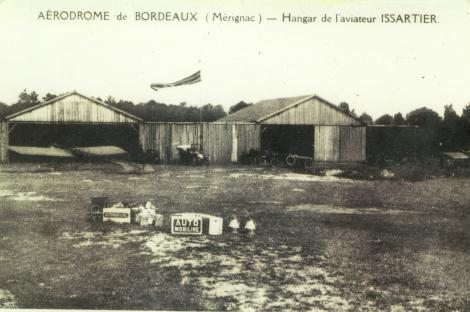
\includegraphics[width=8cm]{Images/premier.jpg}  
      \caption{Aérodrome de Bordeaux-Mérignac}
      \label{fig:aérodrome}
    \end{subfigure}
    \begin{subfigure}{0.5\textwidth}
      \centering
      % include second image
      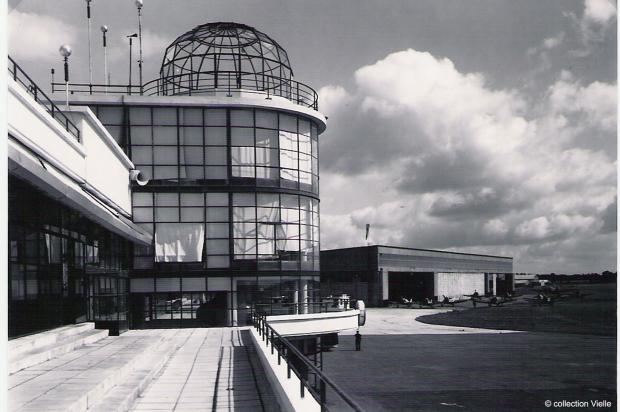
\includegraphics[width=8cm]{Images/premiere_aerogare.jpg}  
      \caption{Première aérogare}
      \label{fig:premiereAerogare}
    \end{subfigure}
\end{figure}


\newpage
De nombreux travaux se succèdent jusqu'en 2003 afin d'agrandir l'aéroport et d'y ajouter de nouveaux halls d'enregistrement et d'embarquements ainsi qu'une tour de contrôle.

En 2007, l'état concède l'exploitation et la gestion de l'aéroport à la SA ADBM pour 30 ans. Depuis, de nombreux travaux ont été réalisés comme la création d'un nouveau parking plus économique et le hall "billi" destiné aux compagnies aériennes low-cost (Ryanair et EasyJet). Il sera par la suite agrandi en 2015.\newline

\begin{figure}[hbt!]
    \begin{subfigure}{0.5\textwidth}
      \centering
      % include first image
      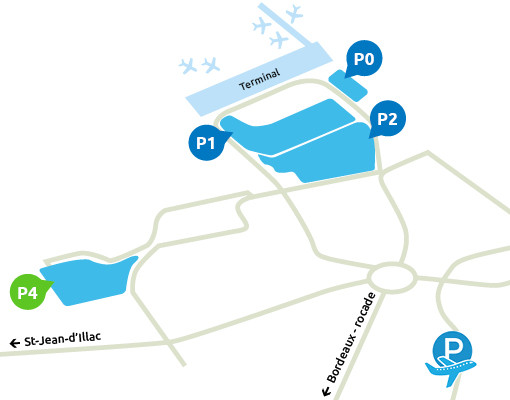
\includegraphics[width=.7\linewidth]{Images/parkings.jpg}  
      \caption{Plan des parkings}
      \label{fig:parking4}
    \end{subfigure}
    \begin{subfigure}{0.5\textwidth}
      \centering
      % include second image
      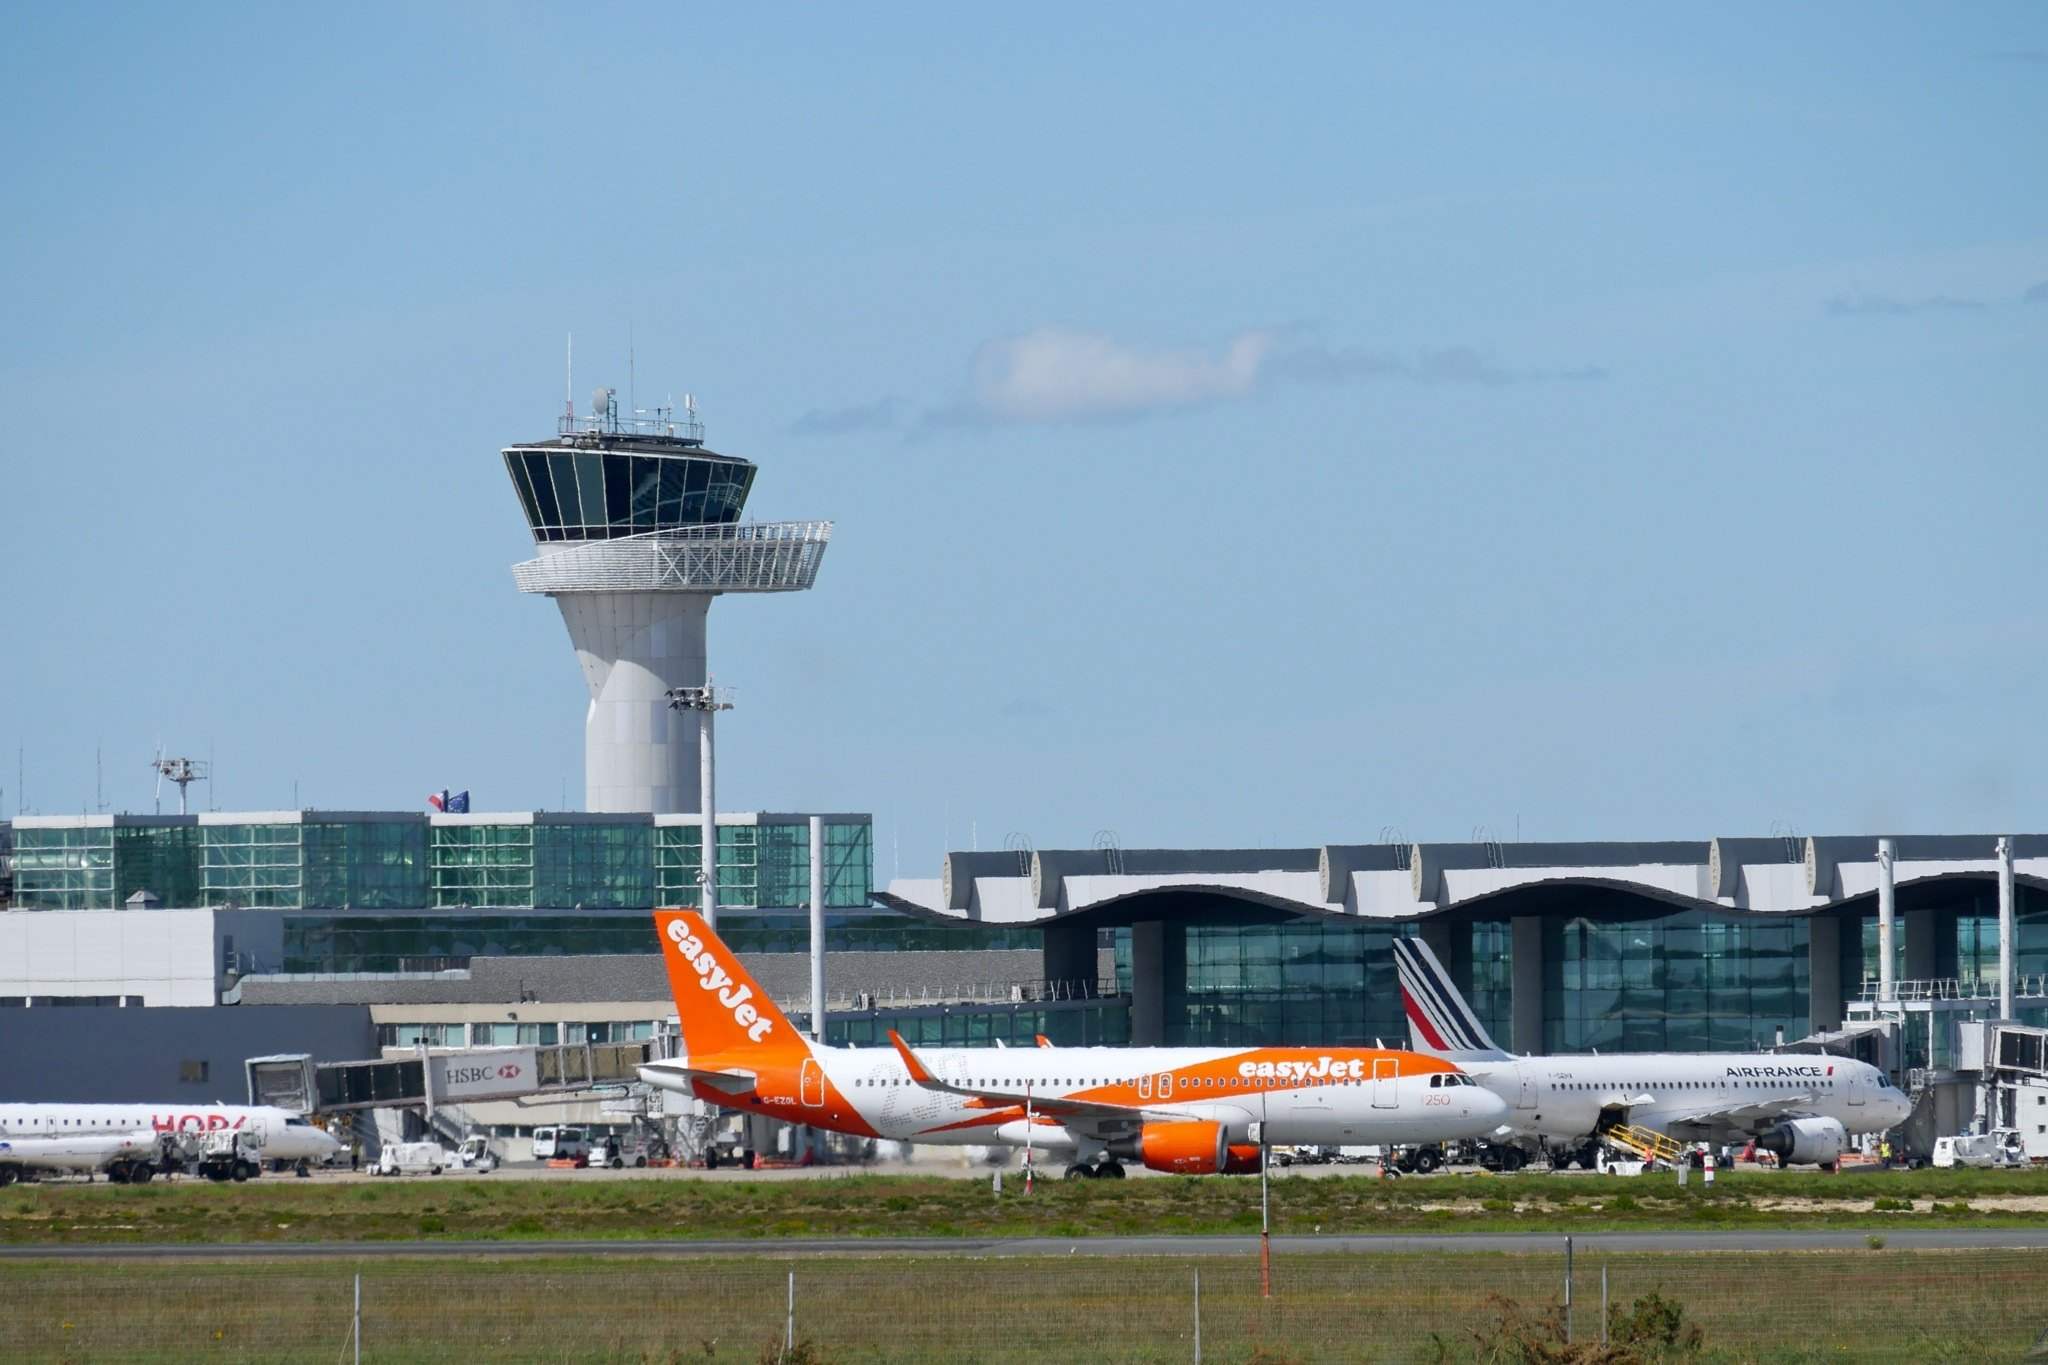
\includegraphics[width=.7\linewidth]{Images/tour.jpg}  
      \caption{Nouvelle Tour de Contrôle}
      \label{fig:tour}
    \end{subfigure}
        
    \begin{subfigure}{.5\textwidth}
      \centering
      % include third image
      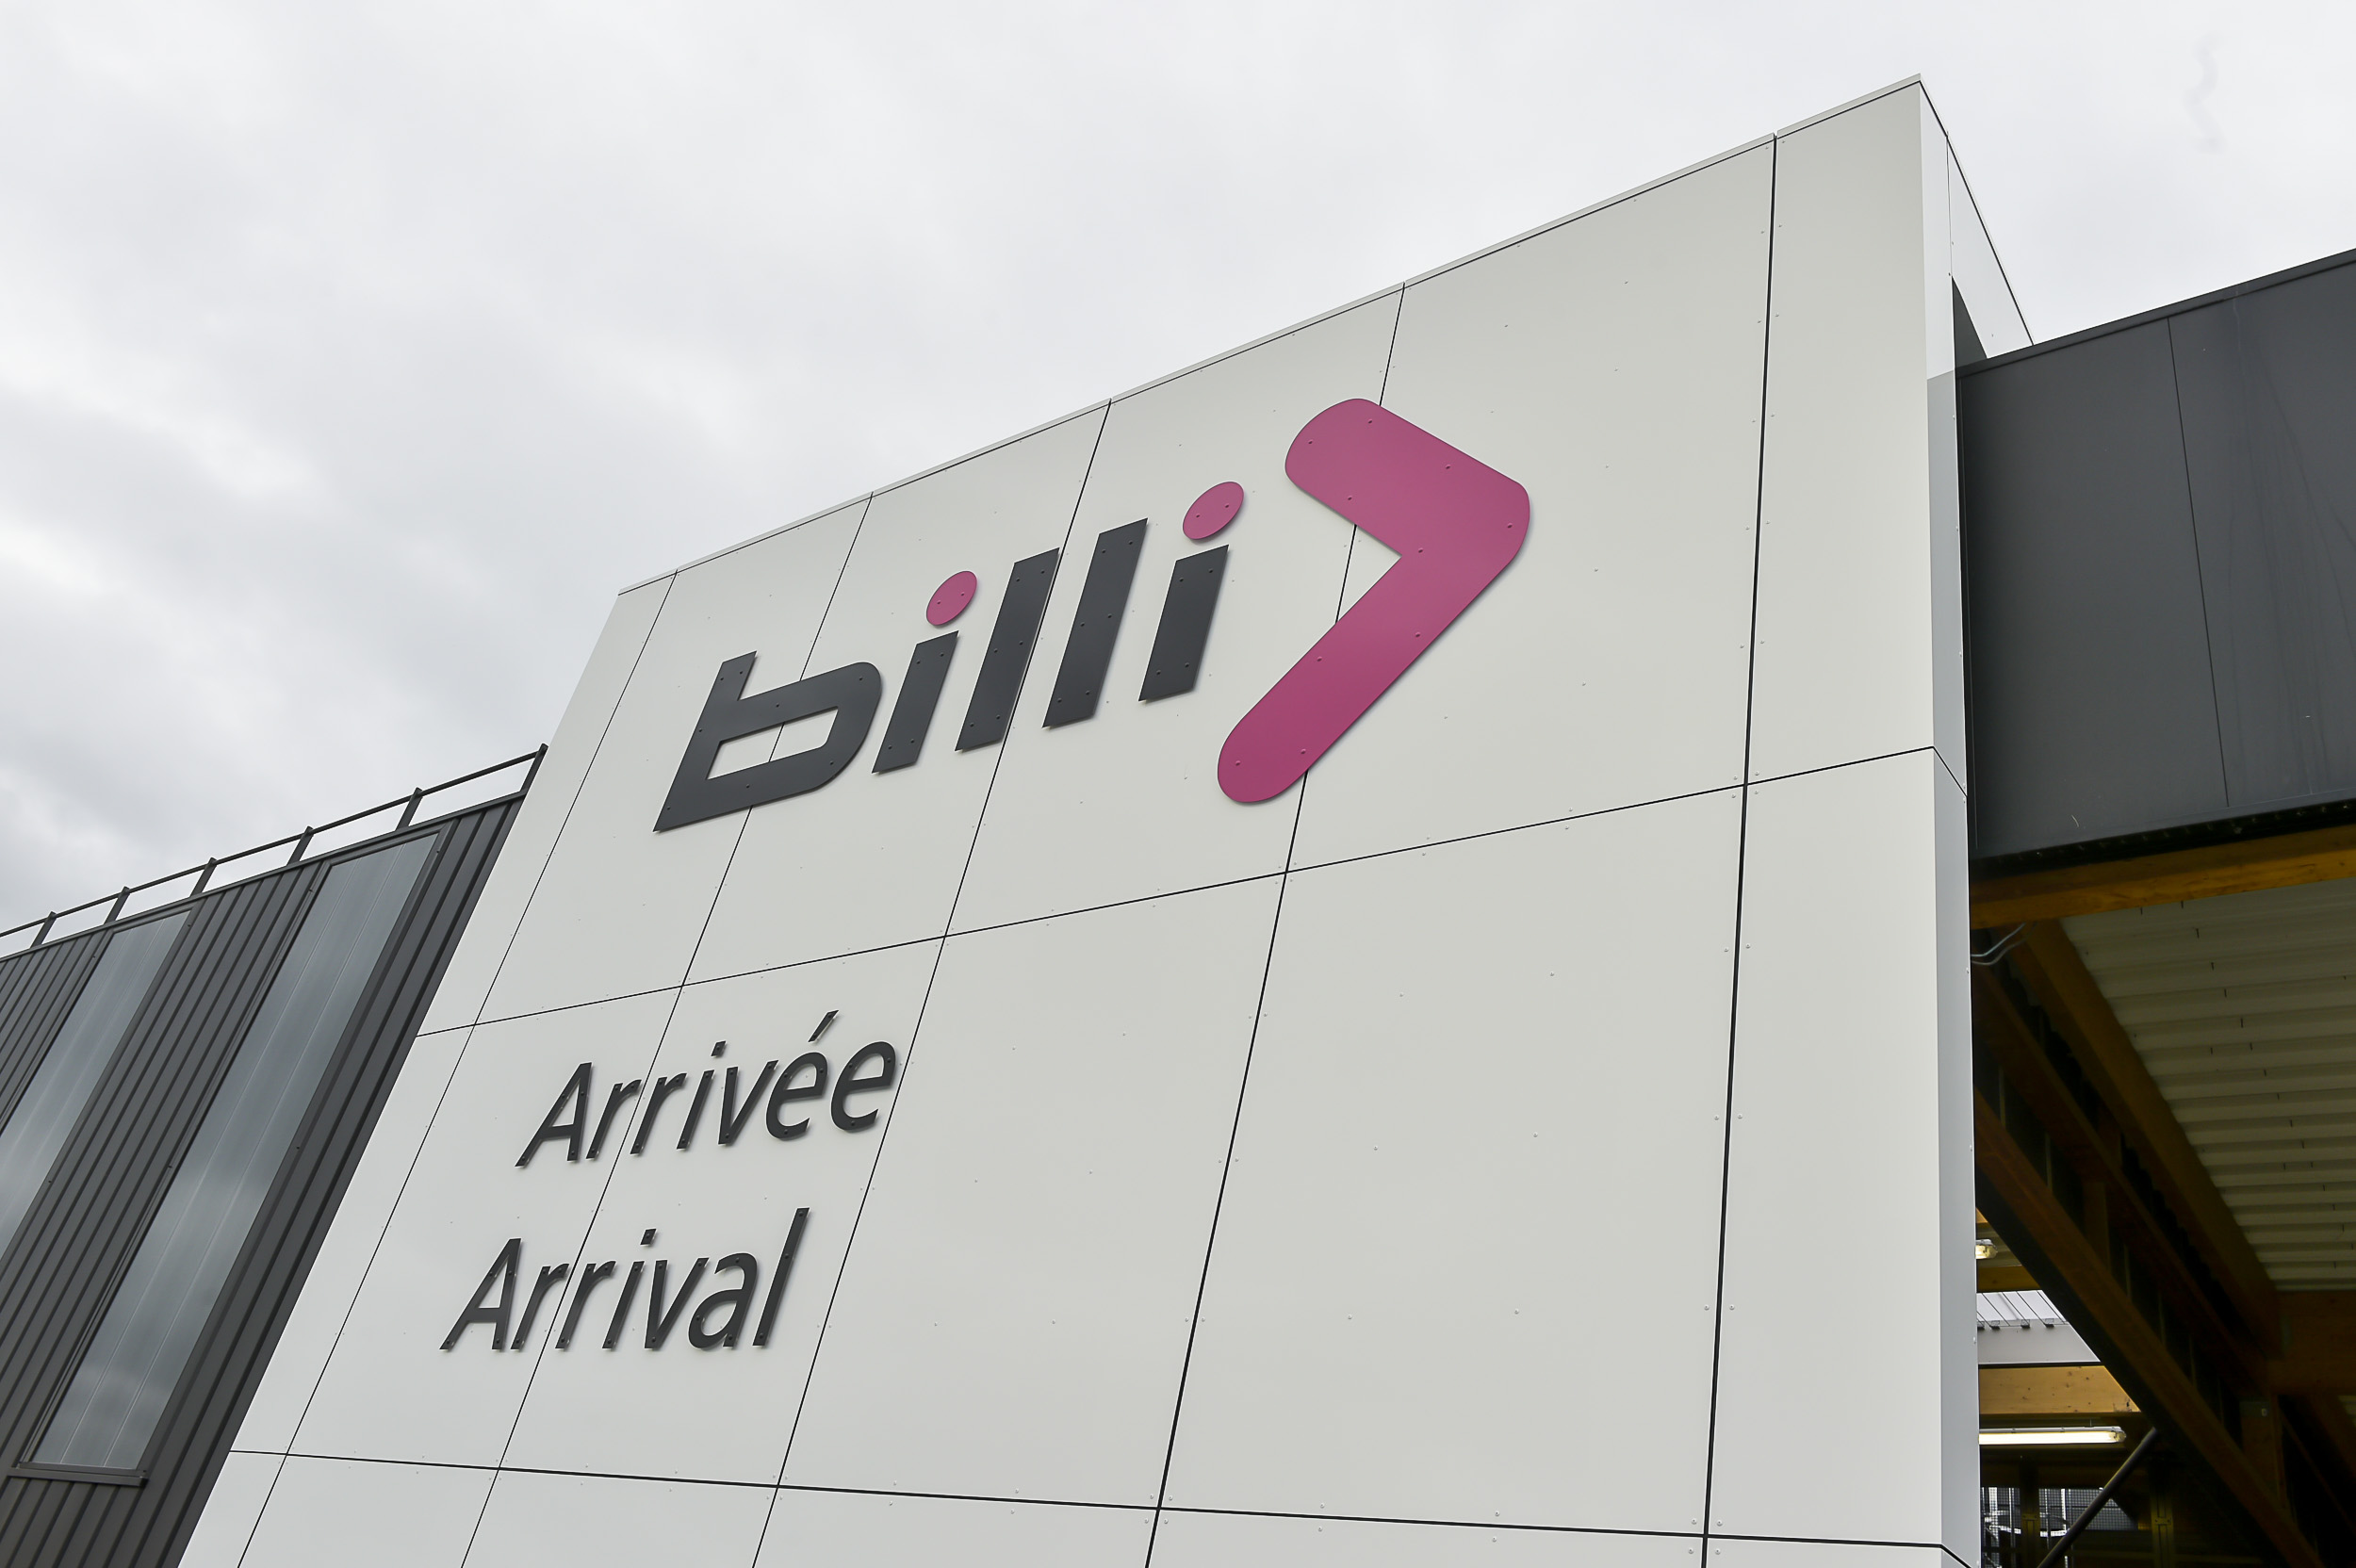
\includegraphics[width=.7\linewidth]{Images/billiext.jpg}  
      \caption{Terminal billi}
      \label{fig:billiext}
    \end{subfigure}
    \begin{subfigure}{.5\textwidth}
      \centering
      % include fourth image
      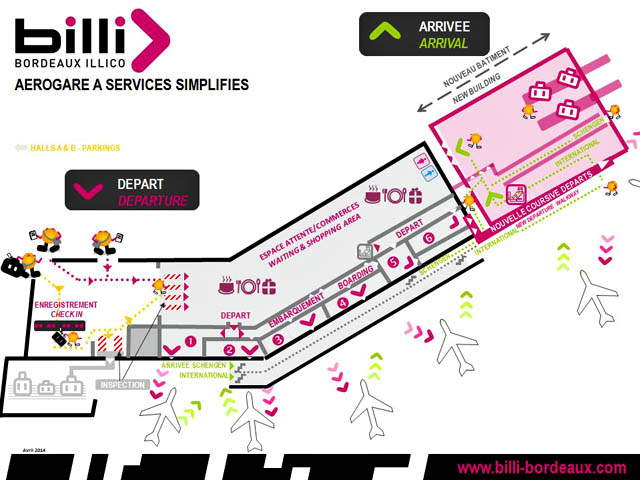
\includegraphics[width=.7\linewidth]{Images/billi.jpg}  
      \caption{Plan billi}
      \label{fig:planBilli}
    \end{subfigure}
    \label{fig:travaux}
\end{figure}

\newpage

\textbf{Infrastructures actuelles}\newline


A ce jour, la SA ADBM gère et exploite toujours l'Aéroport de Bordeaux-Mérignac.
L'aéroport possède aujourd'hui 2 pistes sécantes, 39 portes d'embarquements et 3 terminaux :

\begin{itemize}
    \item Le Hall A : National et International
    \item Le Hall B : National
    \item billi : National et International Low-Cost uniquement (EasyJet et Ryanair)\newline
\end{itemize}

Les Hall A et B possèdent deux niveaux accessibles au public, le niveau 0 pour les arrivées et le niveau 1 pour les départs.

\begin{figure}[hbt!]
    \begin{subfigure}{0.5\textwidth}
      \centering
      % include first image
      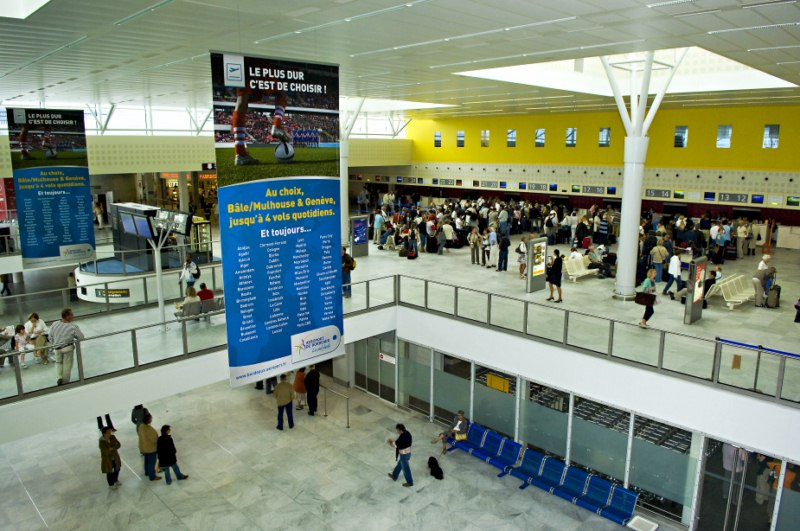
\includegraphics[width=6cm]{Images/inthalla.jpg}  
      \caption{Intérieur Hall A}
      \label{fig:inthalla}
    \end{subfigure}
    \begin{subfigure}{0.5\textwidth}
      \centering
      % include second image
      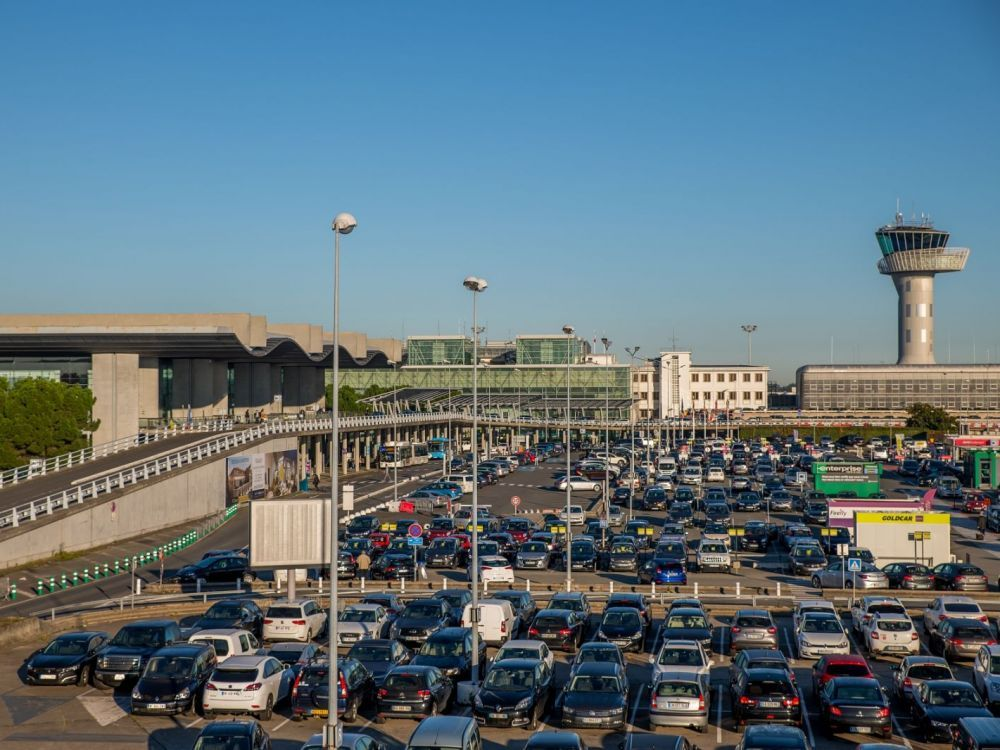
\includegraphics[width=6cm]{Images/exthalla.jpg}  
      \caption{Extérieur Hall A}
      \label{fig:exthalla}
    \end{subfigure}
        
    \begin{subfigure}{.5\textwidth}
      \centering
      % include third image
      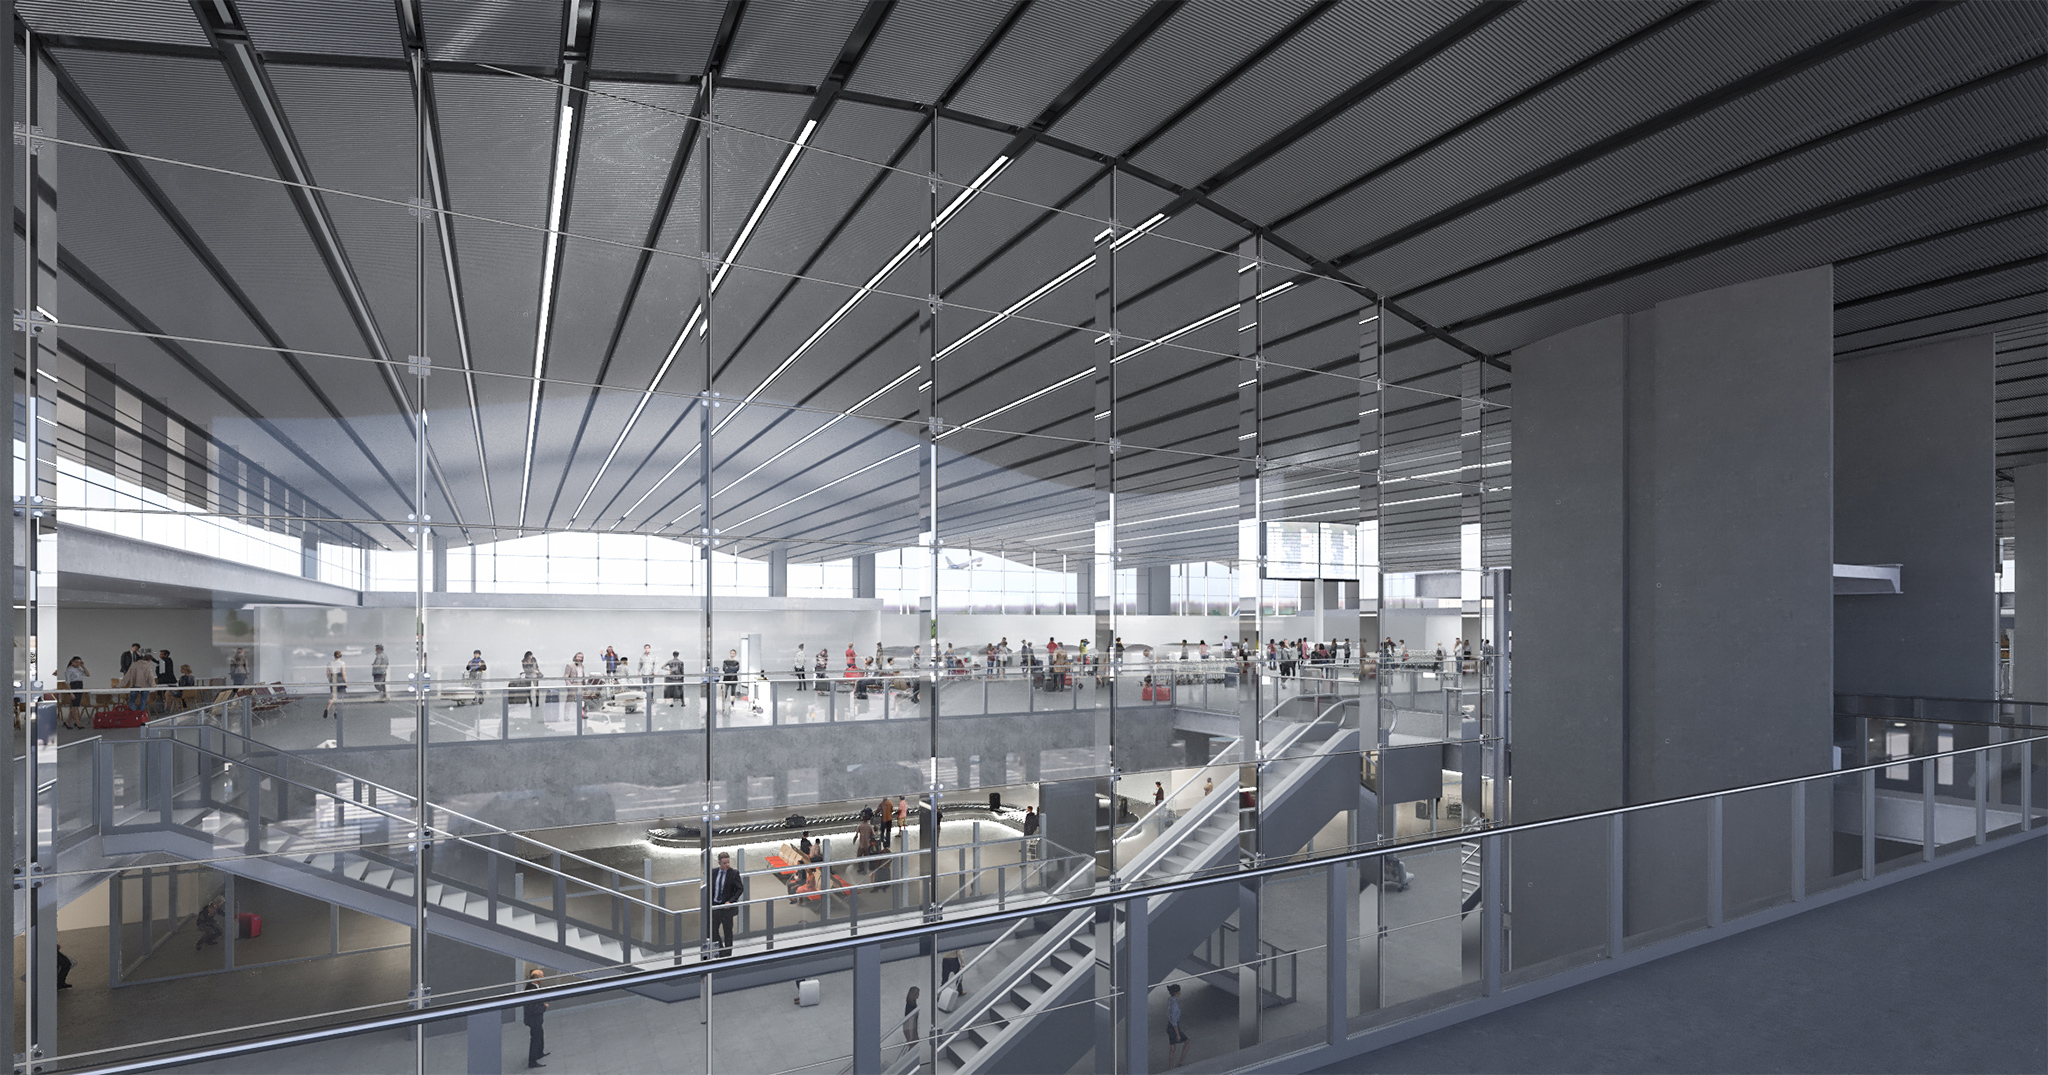
\includegraphics[width=6cm]{Images/inthallb.jpg}  
      \caption{Intérieur Hall B}
      \label{fig:inthallb}
    \end{subfigure}
    \begin{subfigure}{.5\textwidth}
      \centering
      % include fourth image
      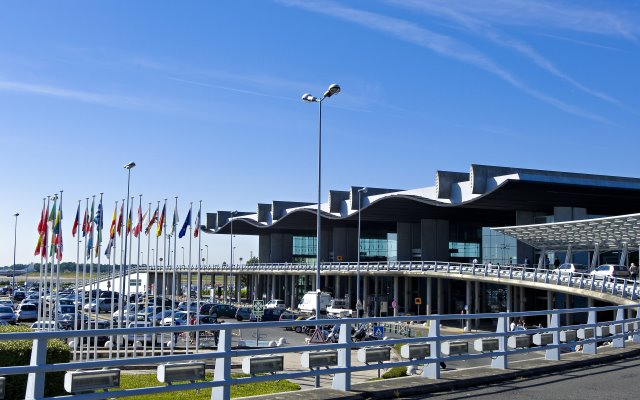
\includegraphics[width=6cm]{Images/exthallb.jpg}  
      \caption{Extérieur Hall B}
      \label{fig:exthallb}
    \end{subfigure}
    \caption{Les différents Halls}
    \label{fig:halls}
\end{figure}

\begin{figure}[hbt!]
    \centering
    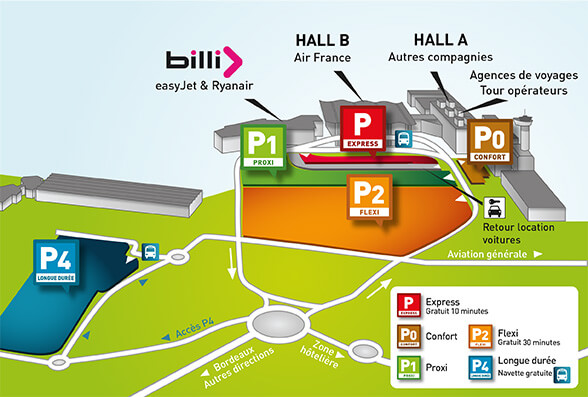
\includegraphics[width=12cm]{Images/plan.jpg}
    \caption{Plan Général}
    \label{fig:plangeneral}
\end{figure}

\newpage

\textbf{Infrastructures futures}\newline

Actuellement, deux plans d'aménagement on été engagés : le Satellite 3 et le prolongement de la ligne A du Tramway.

Le Satellite 3 est un nouveau bâtiment construit côté piste du Hall A afin d'augmenter le nombre de portes d'embarquement pour l'international.

La livraison de ce bâtiment est prévue pour le 13 août 2021.\newline

\begin{figure}[hbt!]
    \centering
    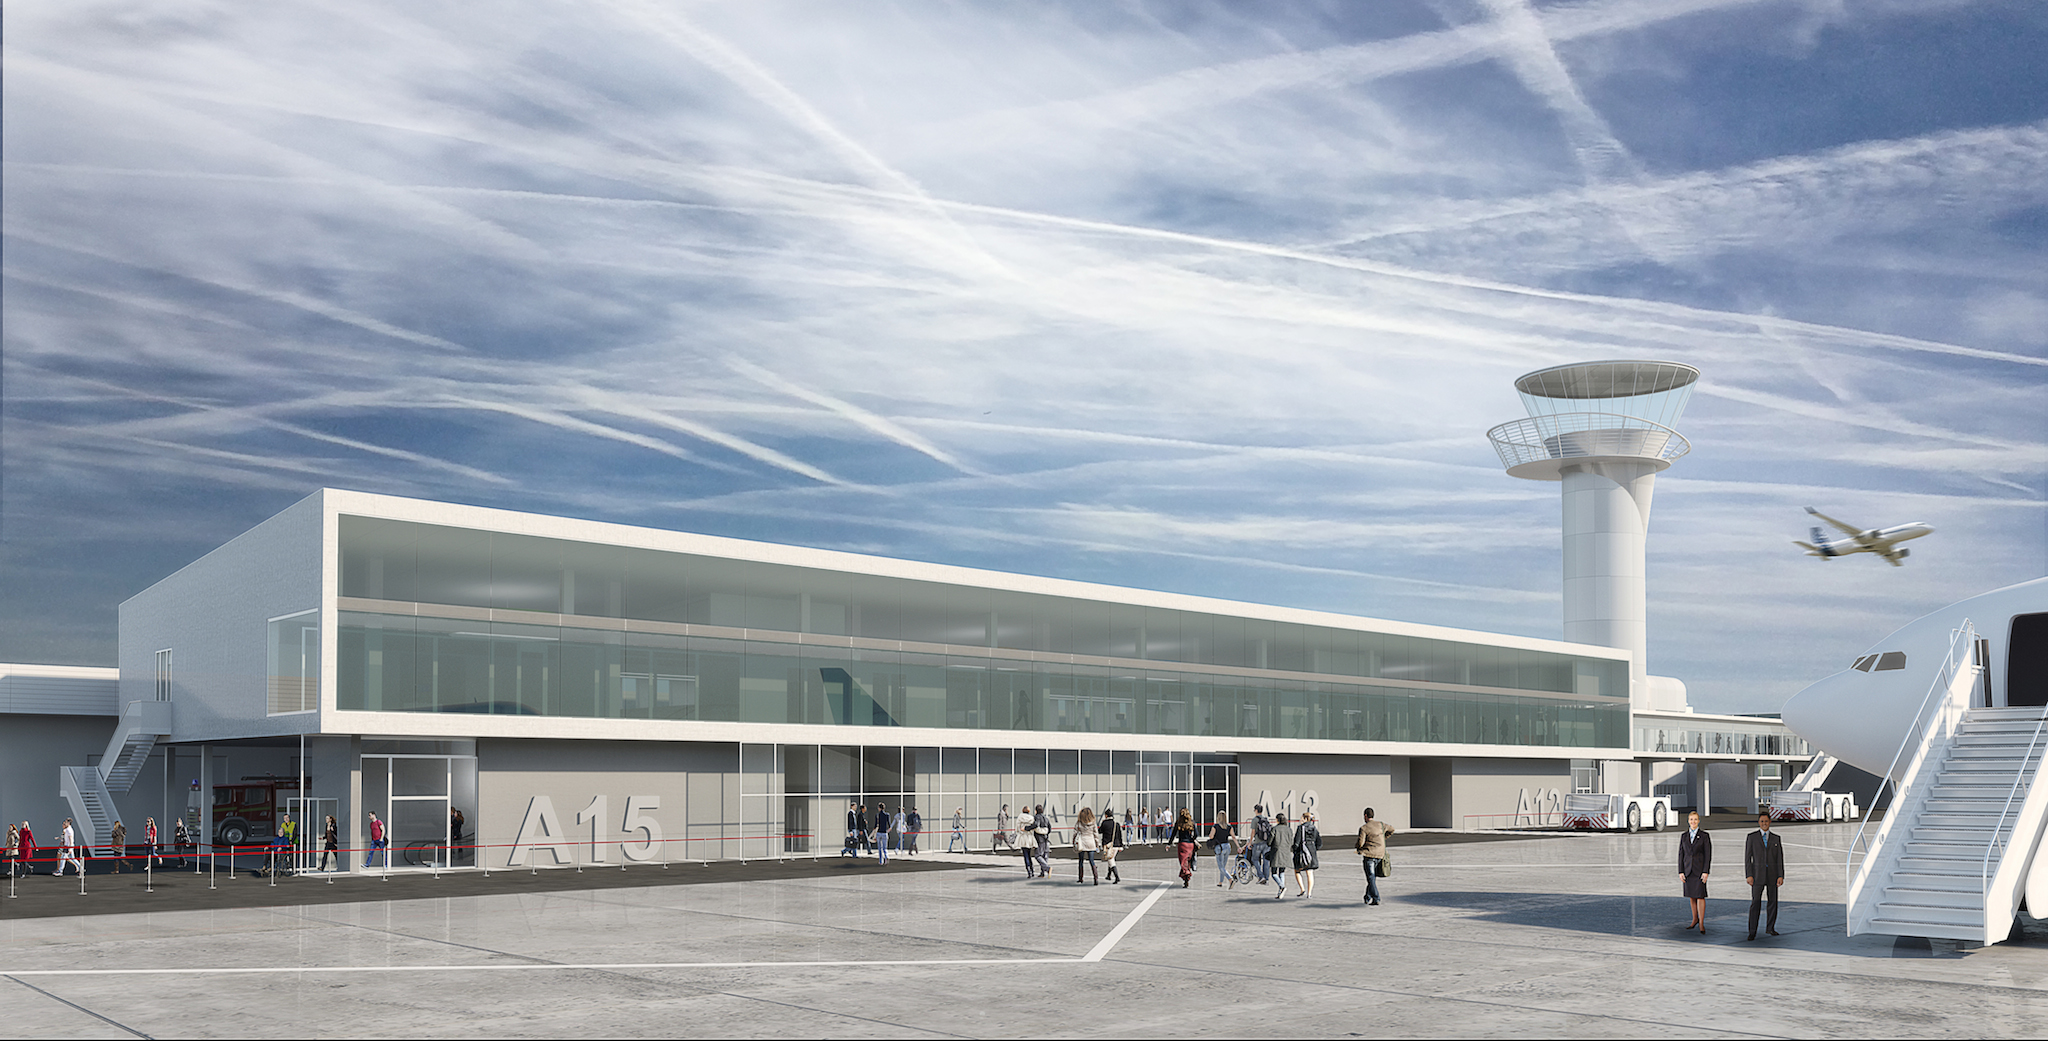
\includegraphics[width=13cm]{Images/satellite3.jpg}
    \caption{Futur Satellite 3}
    \label{fig:sat3}
\end{figure}

En partenariat avec Bordeaux Métropole, la SA ADBM a engagé des travaux qui visent à rendre l'accès à l'aéroport plus simple. La ligne de tramway A est donc prolongée de 6 stations avec le Terminus au pied des aéroports. Ces travaux ont été lancés en 2019 et la livraison est prévue pour l'automne 2022.\newline

\begin{figure}[hbt!]
    \centering
    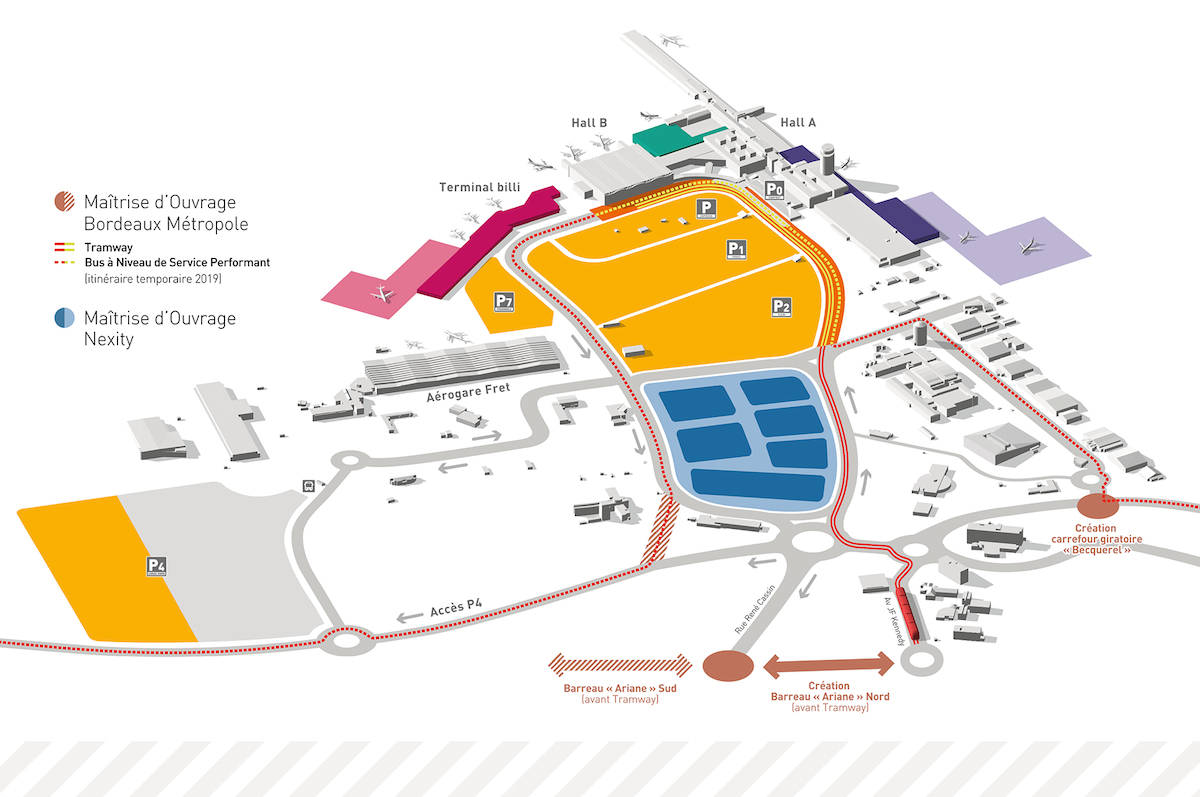
\includegraphics[width=16cm]{Images/tramway.jpg}
    \caption{Plan du futur tramway}
    \label{fig:futurtram}
\end{figure}

\newpage

\textbf{Chiffres clés}\newline

L'aéroport de Bordeaux-Mérignac a fait voyager près de 7,7 millions de passagers en 2019 :

\begin{figure}[hbt!]
    \centering
    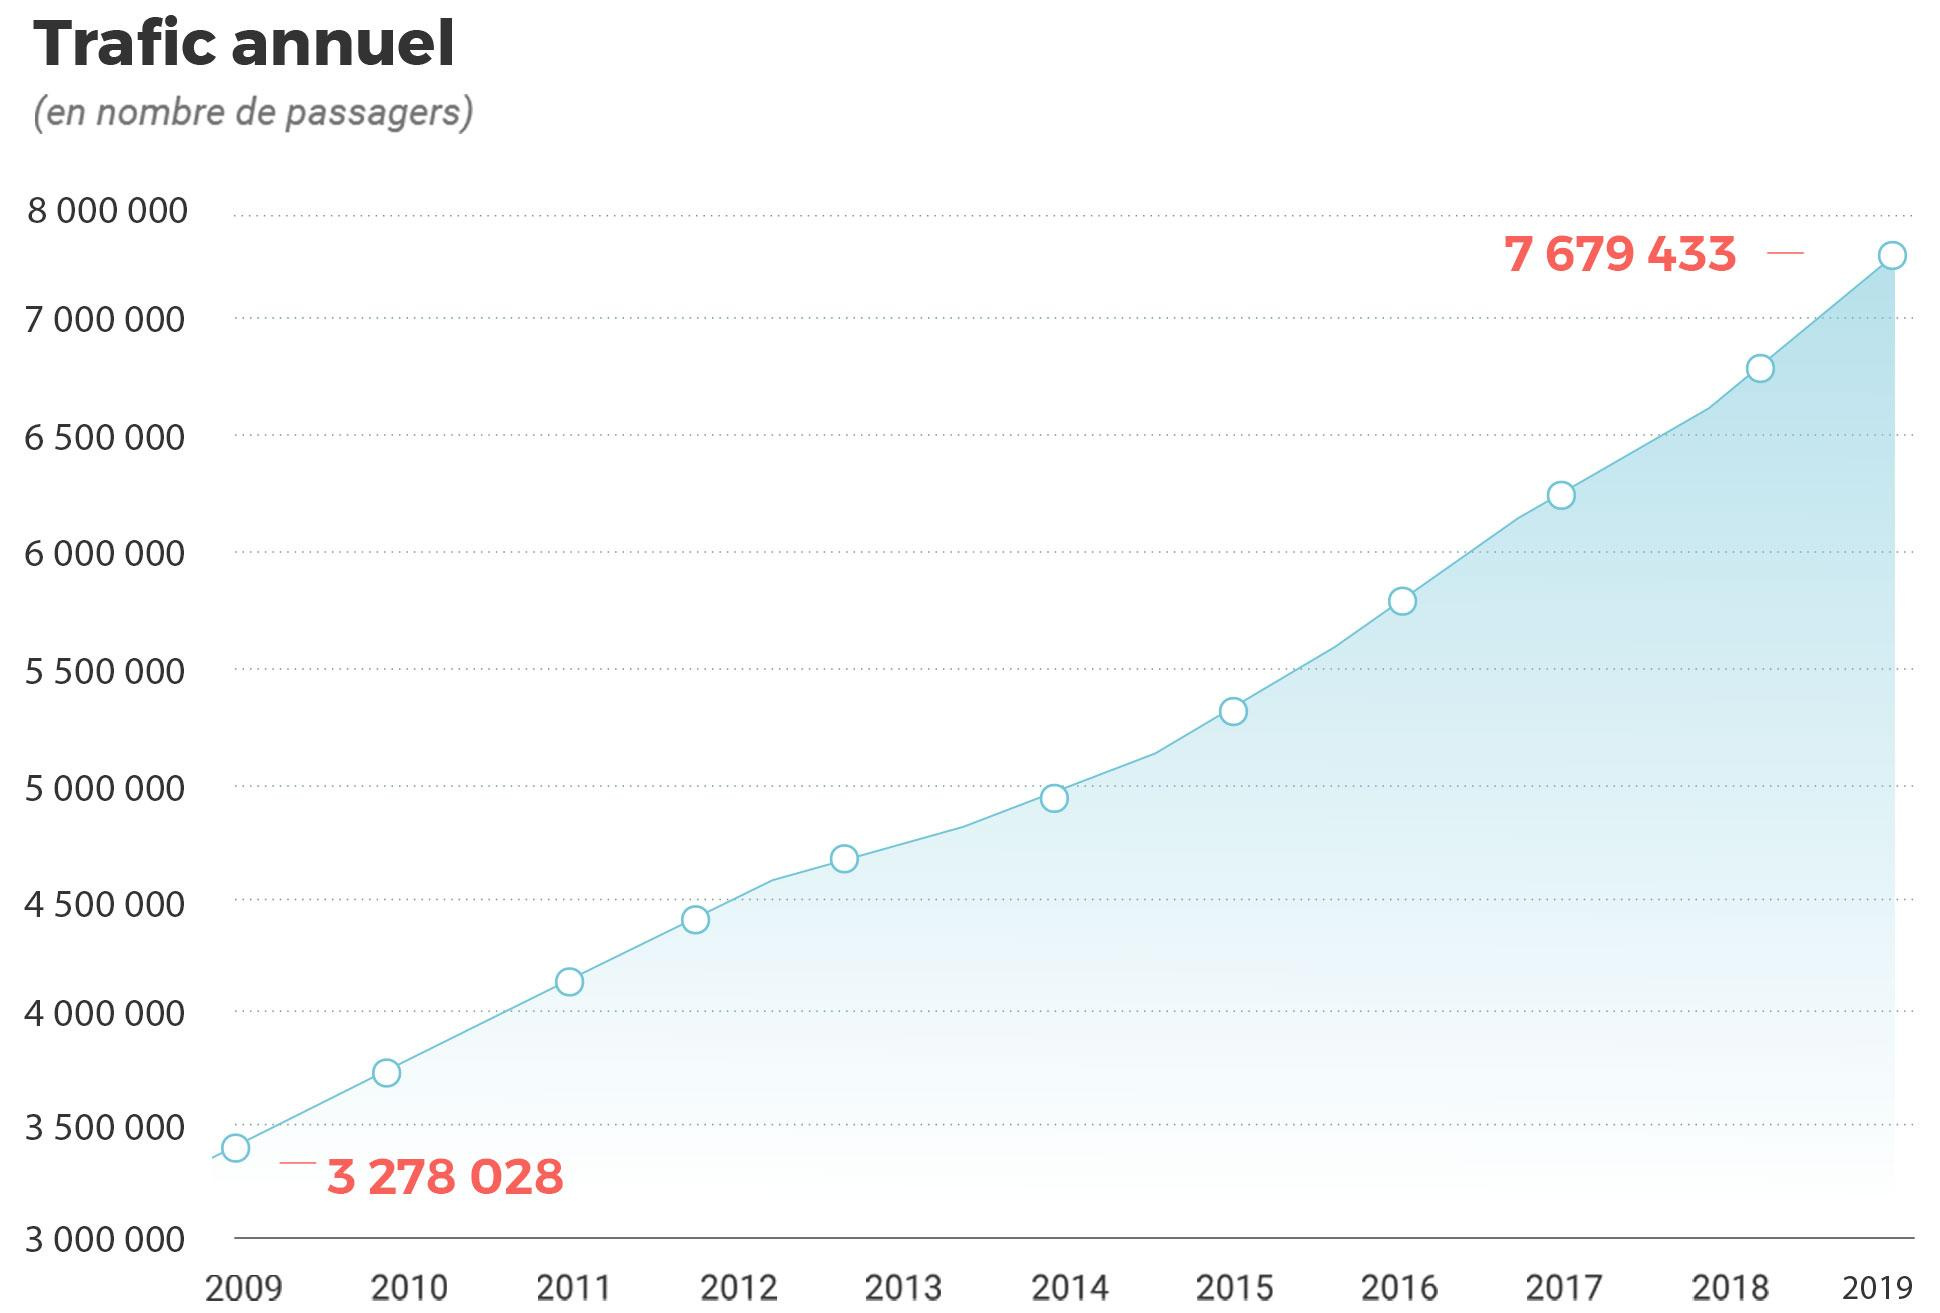
\includegraphics[width=12cm]{Images/trafic.jpg}
    \label{fig:trafic}
\end{figure}

Avant la pandémie de COVID-19, l'aéroport avait pour but de faire voyager 10 millions de passagers en 2023.

En 2019, 34 compagnies aériennes ont opéré des vols, avec un total de 163 lignes directes reliées à 31 pays différents.
De plus, plus de 125 000 tonnes de fret ont été acheminées grâce aux cargos.

C'est également un bassin d'emploi important puisque plus de 8000 personnes travaillent sur la plateforme aéroportuaire (dont 200 à la SA ADBM).
94 établissements sont présents sur site : entreprises, commerces, industries et organismes publics.

\section{Personnes impliquées}


Mon tuteur était Monsieur Serge CLARY, Chef de Projet Informatique, et ma supérieure Madame Nathalie CORDEAU, Chef du Service Organisation, Informatique, Systèmes Industriels au sein du département des opérations techniques.\footnote{Tous les organigrammes disponibles en Annexe}

J'ai travaillé en proche collaboration avec :

\begin{itemize}
    \item Monsieur Marc RIVAULT : Administrateur Systèmes, Réseaux et Bases de données,
    \item Monsieur Gurvan QUENET : Responsable Sécurité des Systèmes d'Information,
    \item Monsieur Kamal MAHAMOUD : Technicien Support Informatique,
    \item Monsieur Yannick FOURNAUD : Administrateur Systèmes, Réseaux et Bases de données, Assistant du Responsable Sécurité des Systèmes d'Information.\newline
\end{itemize}

J'ai également été reçue par :

\begin{itemize}
    \item Monsieur Yannick VALERY : Administrateur Systèmes, Réseaux et Bases de données,
    \item Monsieur Olivier CABANNE : Attaché Relations Riverains et Environnement,
    \item Madame Fabienne COLAS : Coordinatrice Piste,
    \item Madame Christelle DIJOUX : Chargée de Mission SMQS SME\footnote{Système de Management de l'Entreprise, essentiellement de la Qualité (SMQ), de l'Environnement (SME) et de la Sécurité (SMS).}.
\end{itemize}


L'avantage d'une entreprise avec une grande variété de postes, est que j'ai pu constater à quel point l'informatique est essentiel dans tous les services, autant sur l'aspect logiciel que matériel.

\newpage

\section{Missions et tâches réalisées}

Plusieurs types de tâches m’ont été données, à la fois techniques mais également administratives :


Les salariés de l’aéroport étant toujours sur Office 2010, ma première mission a été d’analyser les différences entre Office 2010 et 2019 afin de savoir quel type de formation ou documentation pourrait accompagner la transition, et ensuite de réaliser les supports adéquats. J’ai donc créé un document détaillé de tous les changements entre ces versions, puis ensuite un flyer\footnote{Disponible en annexe} les résumant de manière simplifiée.\newline

Ma seconde mission était de mettre à jour des ordinateurs "Crews", les passer de Windows 7 à Windows 10 en réinstallant d’autres logiciels. Les banques d’enregistrements sont équipées de ces ordinateurs qui permettent d’enregistrer les bagages en soute et d’imprimer leurs identifications à partir d’un scan de la carte d’embarquement du passager. Ces mêmes matériels servent également pour l’accès à la sûreté et en porte d’embarquement. Les passagers scannent leur carte d’embarquement pour que le personnel aéroportuaire ait accès aux informations dont ils ont besoin pour l’embarquement.

J’ai commencé à faire quelques manipulations sur les ordinateurs Crews : mise à jour du BIOS et installation de Windows à partir d’un logiciel de gestion : Ivanti. Cependant je n’ai jamais eu l'occasion de les installer : des problèmes techniques ont été repérés plus tard dans l’installation, et nous avons donc dû suspendre temporairement le projet.

\begin{figure}[hbt!]
  \begin{subfigure}{0.5\textwidth}
    \centering
    % include first image
    
\includegraphics[width=8cm]{Images/logocrews.png}  
    \label{fig:logocrews}
  \end{subfigure}
  \begin{subfigure}{0.5\textwidth}
    \centering
    % include second image
    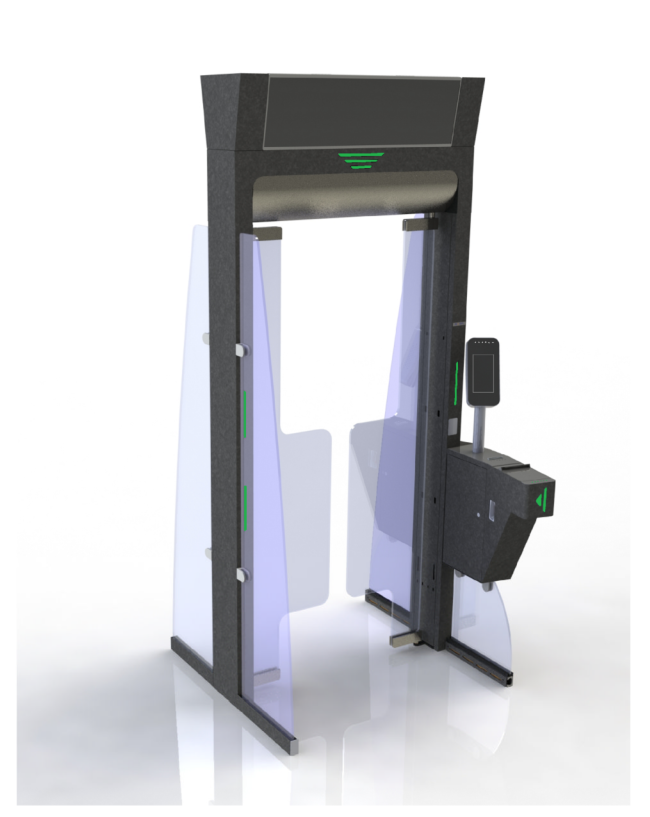
\includegraphics[width=5cm]{Images/crews2.png}\newline  
    \label{fig:portecrews}
  \end{subfigure}
  \caption{Crews en porte d'embarquement}
\end{figure}


J’ai également dû intervenir sur les boîtiers Wyse. Ces boîtiers sont utilisés à l’aéroport comme boîtiers de téléaffichage. Ils servent à afficher notamment les écrans de départs et d’arrivées de vols, les temps d’attente, les destinations sur les portes d’embarquements et banques d'enregistrements bagages. Un modèle plus performant a été acheté et il fallait donc les configurer : mise à jour du BIOS, flash du BIOS, installation de Windows et installation dans le réseau.


J’ai donc effectué ces démarches sur une cinquantaine de postes.\newline

\begin{figure}[hbt!]
  \begin{subfigure}{0.5\textwidth}
    \centering
    % include first image
    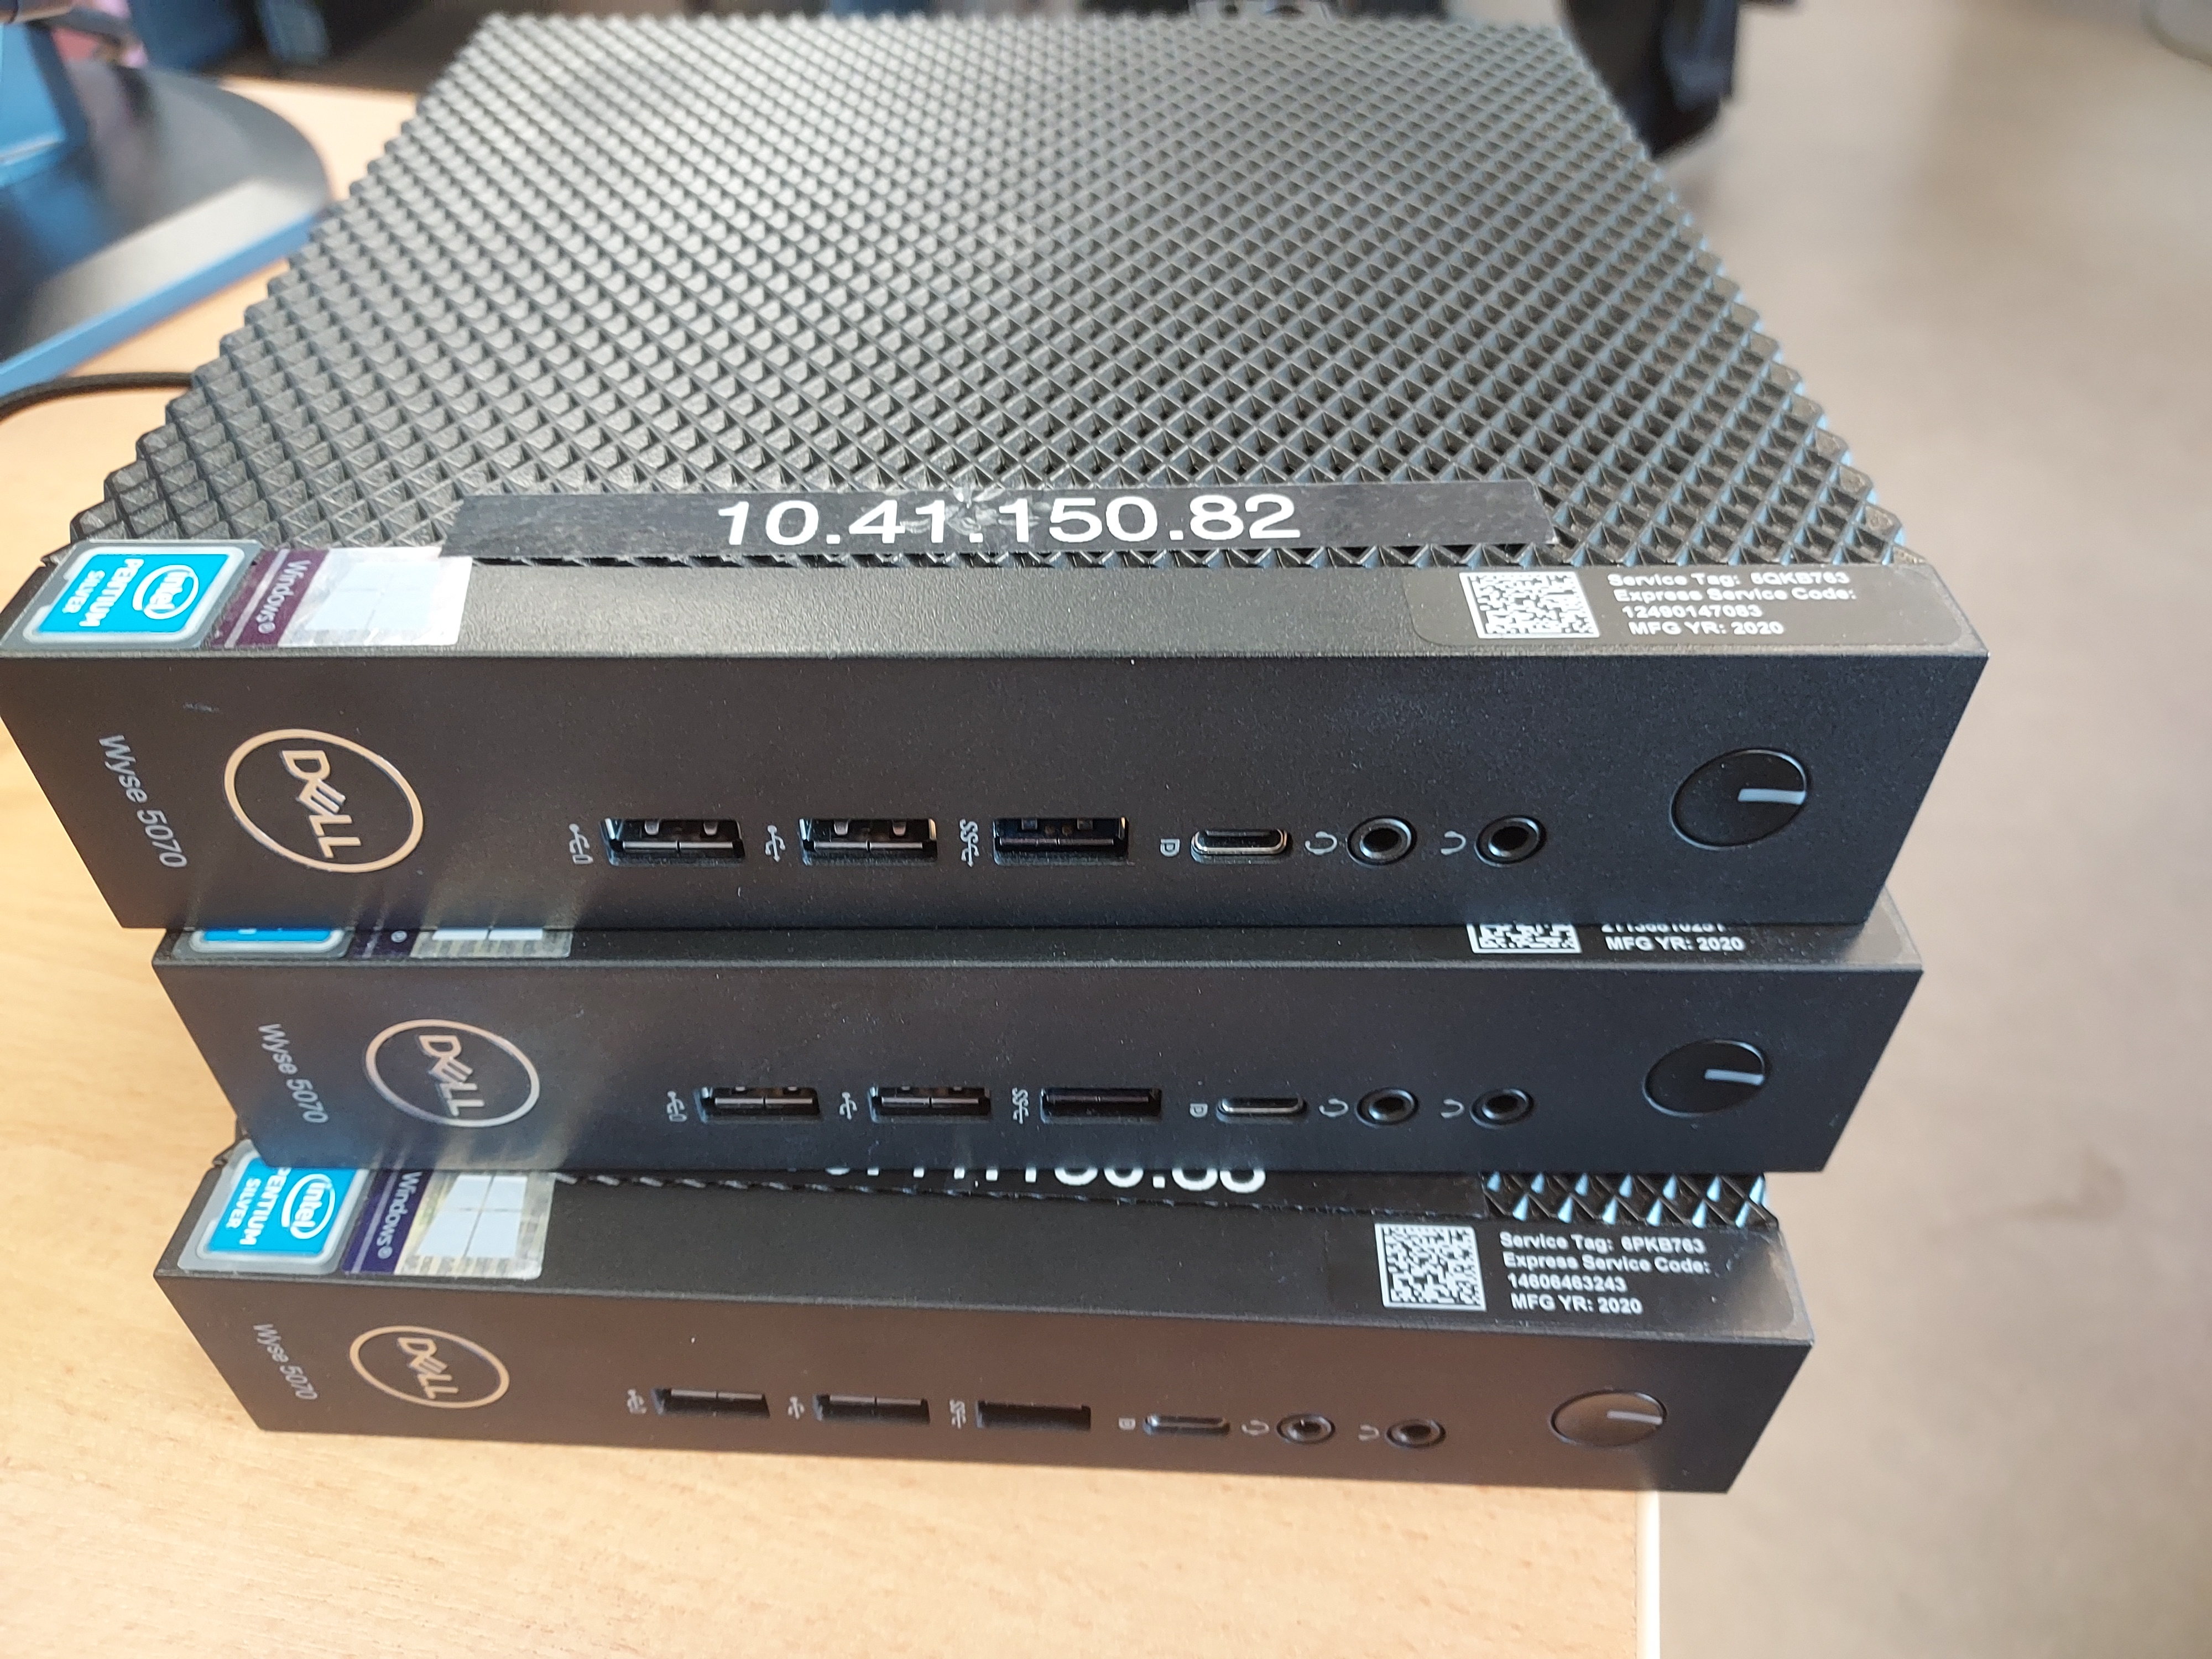
\includegraphics[width=7cm]{Images/wyse.jpg}  
    \label{fig:wyse}
  \end{subfigure}
  \begin{subfigure}{0.5\textwidth}
    \centering
    % include second image
    
\includegraphics[width=7cm]{Images/wyse_logo.jpg}  
    \label{fig:logowyse}
  \end{subfigure}
  \caption{Boîtiers Wyse}
\end{figure}

Durant le premier confinement, certains salariés se sont vus attribués un ordinateur portable afin de faire du télétravail. Une de mes missions était de passer dans tous les bureaux de l’aéroport et de recenser le matériel présent dans ceux-ci puis de comparer avec celui prêté dans la base de données afin de vérifier que tout le personnel a bien ramené les outils prêtés. Au final, il m'a fallu produire un inventaire.\newline


Pour ma dernière mission, toujours concernant le prêt de matériel durant le confinement, plusieurs vols ont été constatés chez ces personnes. Au délà de la perte financière, la perte du disque dur représentait une perte d’informations internes et donc un problème de sécurité. Il fallait donc régler le problème afin de ne pas risquer une fuite de données. Le Responsable Sécurité des Systèmes d’Information et ses supérieurs ont optés pour CRYHOD.


CRYHOD est un logiciel de cryptage de données de disques durs. Gurvan QUENET, le Responsable Cybersécurité de l’aéroport m’a donc donné la mission d’installer ce logiciel sur les ordinateurs portables des salariés afin de sécuriser les disques durs et protéger les données de l’aéroport. J’ai pu l’effectuer sur les postes de mon service, mais je n'ai pas eu le temps de continuer sur ceux de l'ensemble du personnel. Sur la consigne de Monsieur Gurvan QUENET, j'ai donc du, avant mon départ, former mon collègue Monsieur Kamal MAHAMOUD à cette installation afin qu'il la termine après mon départ.

\begin{figure}[hbt!]
  \centering
  
\includegraphics[width=5cm]{Images/logo_cryhod.png}
  \label{fig:logocryhod}
\end{figure}


\newpage

\section{Démarche Responsabilité Sociale de l’Entreprise}


Lorsque l'on pense à un aéroport ou même au milieu aéronautique en général, on ne l'associe pas à une bonne gestion de l'environnement.
Et pourtant, comme toute entreprise, l'Aéroport de Bordeaux-Mérignac pratique une politique RSE.

J'ai pu rencontrer un des responsables du Service Environnement et Relations Riverains : Monsieur Olivier CABANNE.

En effet, l'entreprise se rend compte que ses activités sont des nuisances pour les riverains et l'environnement. 

La Commission Consultative de l’Environnement (CCE) est l’instance de référence consultée sur toute question d’importance relative à l’aménagement ou à l’exploitation de l’Aéroport de Bordeaux pouvant avoir une incidence sur l’environnement. Ces réunions rassemblent : 

\begin{itemize}
  \item Le Service Environnements et Relations Territoriales de l'Aéroport de Bordeaux-Mérignac,
  \item Les Élus Locaux,
  \item Les Associations de Riverains.
\end{itemize}

Suite à ces réunions, SA ADBM propose de nombreuses solutions.\newline

\textbf{Riverains}\newline

Plusieurs actions ont été menées afin de réduire au maximum la gêne occasionée par les activités aériennes, comme la mise en place d'Aérovision.

\begin{figure}[hbt!]
  \centering
  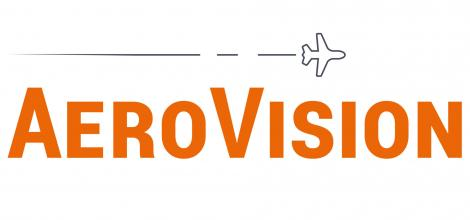
\includegraphics[width=4cm]{Images/logo_aerovision.jpg}
  \label{fig:logoaerovision}
\end{figure}

La majorité des plaintes sont relatives au bruit occasioné par les aéronefs qui volent à basse altitude afin d'atterir ou de décoller.
Les bruits des aéronefs sont soumis à une loi, le bruit capté au sol ne doit pas dépasser les 70 dB. Plusieurs associations de riverains se plaignaient que certains avions dépassaient cette réglementation.\newline

Le service informatique a donc créé AEROVISION. Ils ont installé des stations de mesure de bruit dans des endroits habités dans l'axe des pistes.


Cet outil accessible en ligne est une carte de l'aéroport et de ses environs avec la représentation des stations ainsi que leur bruit mesuré lorsqu'un avion passe au dessus. Les trajectoires vertes sont les arrivées, et bleues les décollages.

\begin{figure}[hbt!]
  \centering
  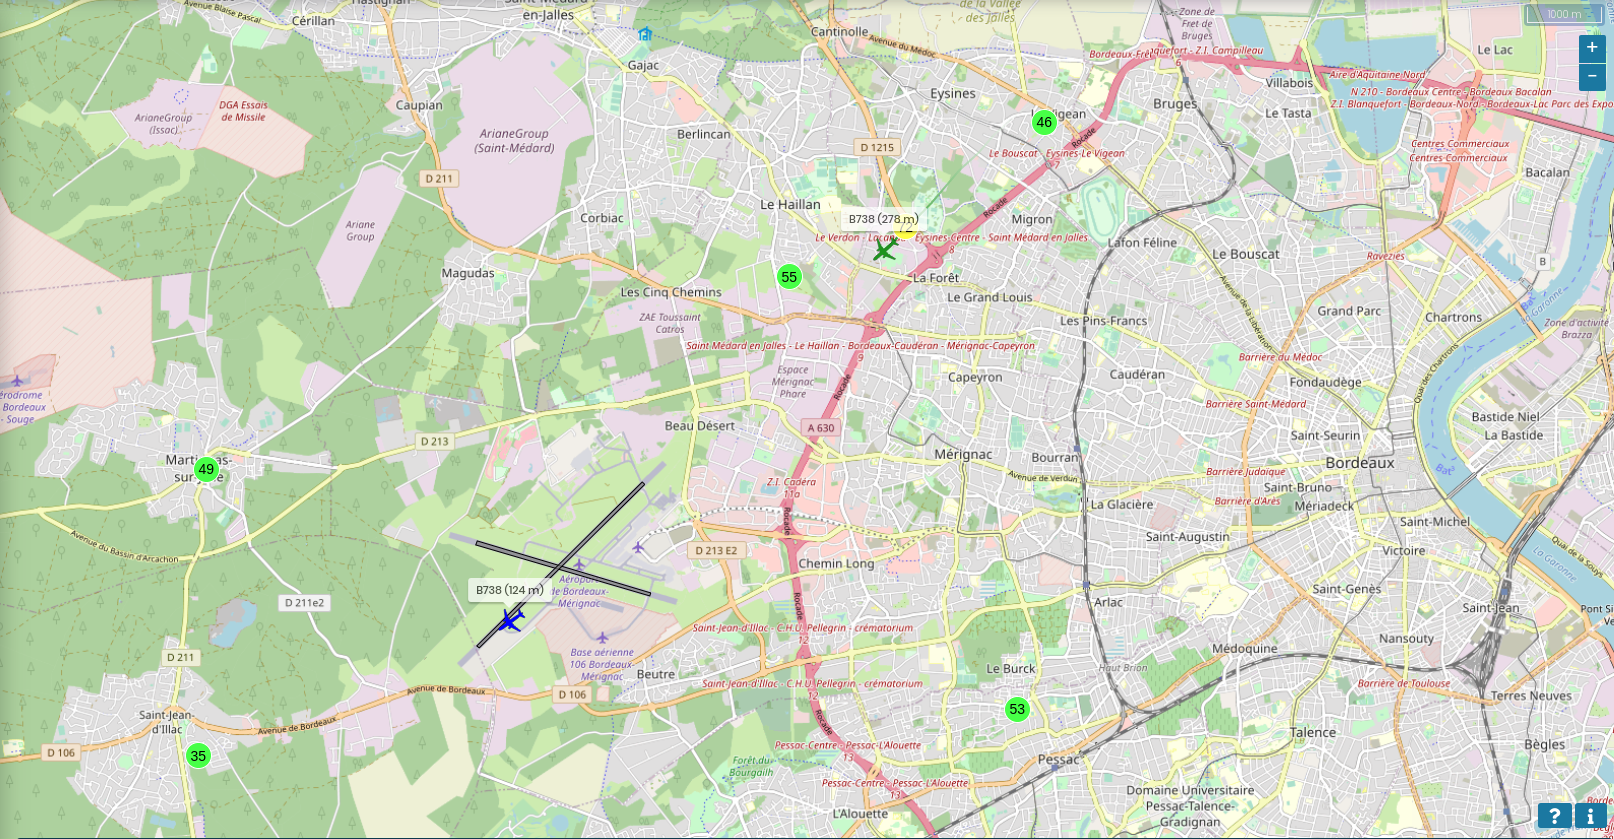
\includegraphics[width=16cm]{Images/aerovision.png}\newline
  \caption{Interface}
  \label{fig:interfaceaerovision}
\end{figure}

Un mode "Historique" est également disponible : grâce à une sélection de 30 minutes, l'utilisateur peut vérifier les informations sur des vols antérieurs.

Pour des raisons de sécurité, AEROVISION a 30 minutes de décalage avec la réalité et n'affiche que les vols civils.

L'outil AEROVISION est disponible à l'adresse : https://trajectoires.bordeaux.aeroport.fr/appmap\newline

De plus, en cliquant sur un avion sur la carte on peut obtenir des informations sur celui-ci : type d'appareil, compagnie, trajectoire, informations d'approche et bruit total.
Une autre fonctionnalité a été créé pour les riverains : "Mon Habitation". Cette fonctionnalité permet de placer sa maison sur la carte grâce à la géolocalisation ou simplement en cliquant sur la carte et d'afficher le point de bruit maximum par rapport à l'habitation.

\begin{figure}[hbt!]
  \begin{subfigure}{0.5\textwidth}
    \centering
    % include first image
    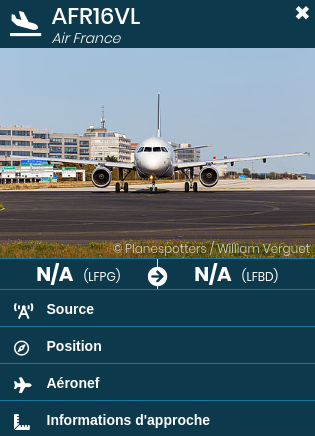
\includegraphics[width=5cm]{Images/aerovisioninfo.png}  
    \caption{Menu Informations Aéronefs}
    \label{fig:aerovisioninfo}
  \end{subfigure}
  \begin{subfigure}{0.5\textwidth}
    \centering
    % include second image
    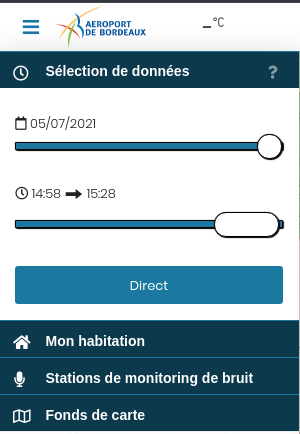
\includegraphics[width=5cm]{Images/aerovisionmaison.png}  
    \caption{Menu "Mon Habitation"}
    \label{fig:aerovisionmaison}
  \end{subfigure}
\end{figure}

Un dispositif d'aide a également été créé : L'aide à l'insonorisation.
C'est une aide financière destinée aux habitants des quatres communes touchées par ce problème : Mérignac, Le Haillan, Eysines et Saint-Jean-d'Illac. Elle prend en charge complètement les travaux de rénovation pour insonoriser l'hôtel ou le logement.

Pour bénéficier de cette aide financière, il faut être situé dans une des zones du Plan de Gêne Sonore en vigueur, et avoir un permis de construire datant d'avant la création du Plan d'Exposition au Bruit.\footnote{Les deux plans sont disponibles plus grands en annexe}
Le but étant de dédommager les personnes s'étant installées près de l'aéroport avant l'augmentation signicative du traffic aérien.

\begin{figure}[hbt!]
  \centering
  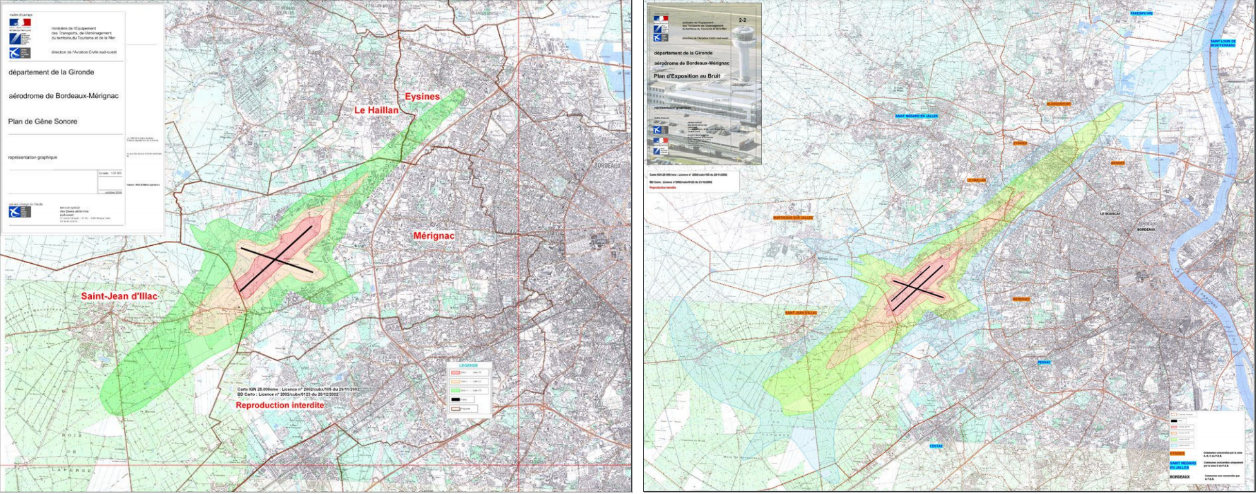
\includegraphics[width=17cm]{Images/pgs_peb.png}\newline
  \caption{Plan de Gêne Sonore et Plan d'Exposition au Bruit}
  \label{fig:pgs_peb}
\end{figure}


Une autre action a été effectuée pour les riverains. La ville de Saint-Jean-D'Illac est située juste en dessous de la trajectoire de décollage de la piste la plus utilisée. Les riverains ont demandés à ce qu'un changement de trajectoire soit envisagé.

Le sujet a été étudié longuement et un problème majeur a été rencontré : si les aéronefs changeaient leurs trajectoires, ils devraient survoler une zone militaire, or cela est strictement interdit.
Une trajectoire alternative a toutefois été trouvée mais il a ensuite fallu effectuer une demande aux services de l'état concernés, et au bout d'un an et demi cela a été accepté.\newline

Aujourd'hui, les avions remontant vers le nord effectuent leur virage bien plus au sud, et contournent donc la ville de Saint-Jean-D'Illac.\newline

\begin{figure}[hbt!]
  \centering
  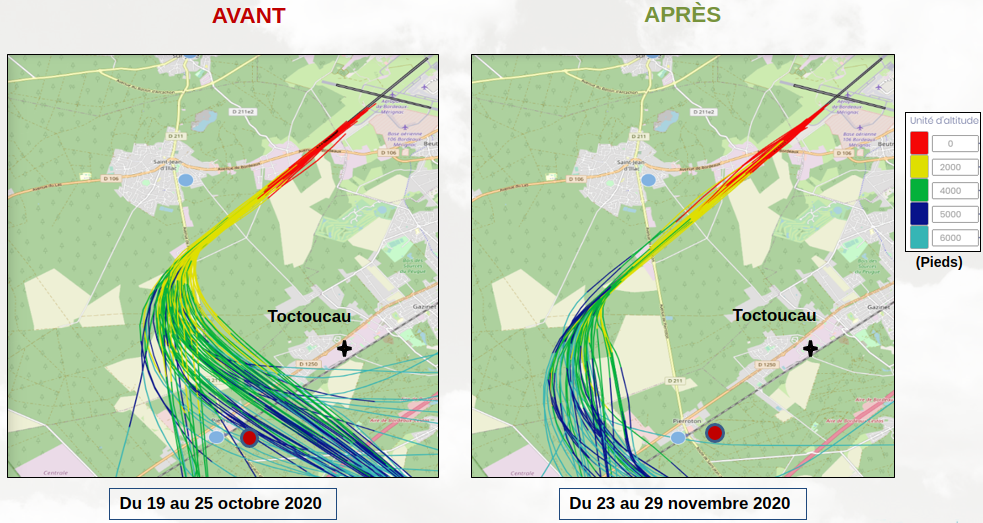
\includegraphics[width=13.5cm]{Images/trajectoires_avant_apres.png}\newline
  \caption{Différentes Trajectoires}
  \label{fig:trajectoires}
\end{figure}

Des mesures audios ont ensuite été réalisées sur les stations de bruit concernées afin de constater ou non des changements.

\begin{figure}[hbt!]
  \centering
  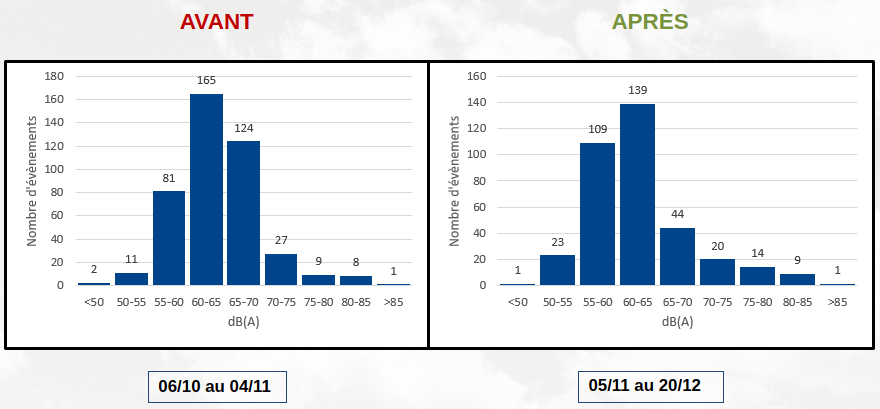
\includegraphics[width=14cm]{Images/bruit_avant_apres.png}\newline
  \label{fig:Mesures audios}
\end{figure}

De plus, pour répondre aux attentes des riverains, l'Aéroport essaie de réduire les vols de nuit qui sont très gênants. Cependant ce n'est pas une tâche aisée puisque cela concerne également l'Aéroport de destination ou de provenance du vol. Des discussons sont actuellement en cours avec certaines compagnies pour trouver des solutions pérennes qui satisferont l'ensemble des parties.\newline


Une dernière action est menée pour améliorer la vie des riverains : trajectoires. C'est un bulletin d'information trimestriel\footnote{Exemplaire du premier trimestre 2021 disponible en annexe} qui leur est destiné dans lequel l'aéroport évoque les problématiques environnementales qui les concerne : mouvement des raffales, statistiques sur les mesures de bruit, décollage et atterisage des aéronefs et la qualité de l'air.


\textbf{Environnement}\newline

Le milieu aérien est un domaine perçu comme très polluant par le grand public et SA ADBM le sait. Un service est consacré à l'environnement. Ils travaillent sur différents points comme les émissions carbones, la faune et flore environnante mais également d'autres sujets.


Au niveau national, des lois ont été mises en places au niveau des compagnies aériennes. Par exemple, un passager peut s'il le souhaite choisir de compenser son émission carbone grâce à un don d'une valeur dépandant de la distance effectuée.
Une partie de cet argent est par la suite utilisée pour acheter des avions moins polluants ou reversé aux aéroports afin de réduire les émissions de la plateforme.\newline

La SA ADBM prend ces enjeux très au sérieux : en effet, 8 millions d'euros ont été attribués pour réduire l'impact négatif sur l'environnement.
L'entreprise a également rejoint le programme Airport Carbon Accreditation (ACA). L'objectif de ce programme international est de rendre les plateformes aéroportuaires neutres en émissions carbone.
L'Aéroport de Bordeaux-Mérignac a validé le niveau 1 le 11 juin 2021. L'objectif de neutralité carbone est prévu pour 2030\footnote{Les étapes du programme sont disponibles en annexe}.

\begin{figure}[hbt!]
  \centering
  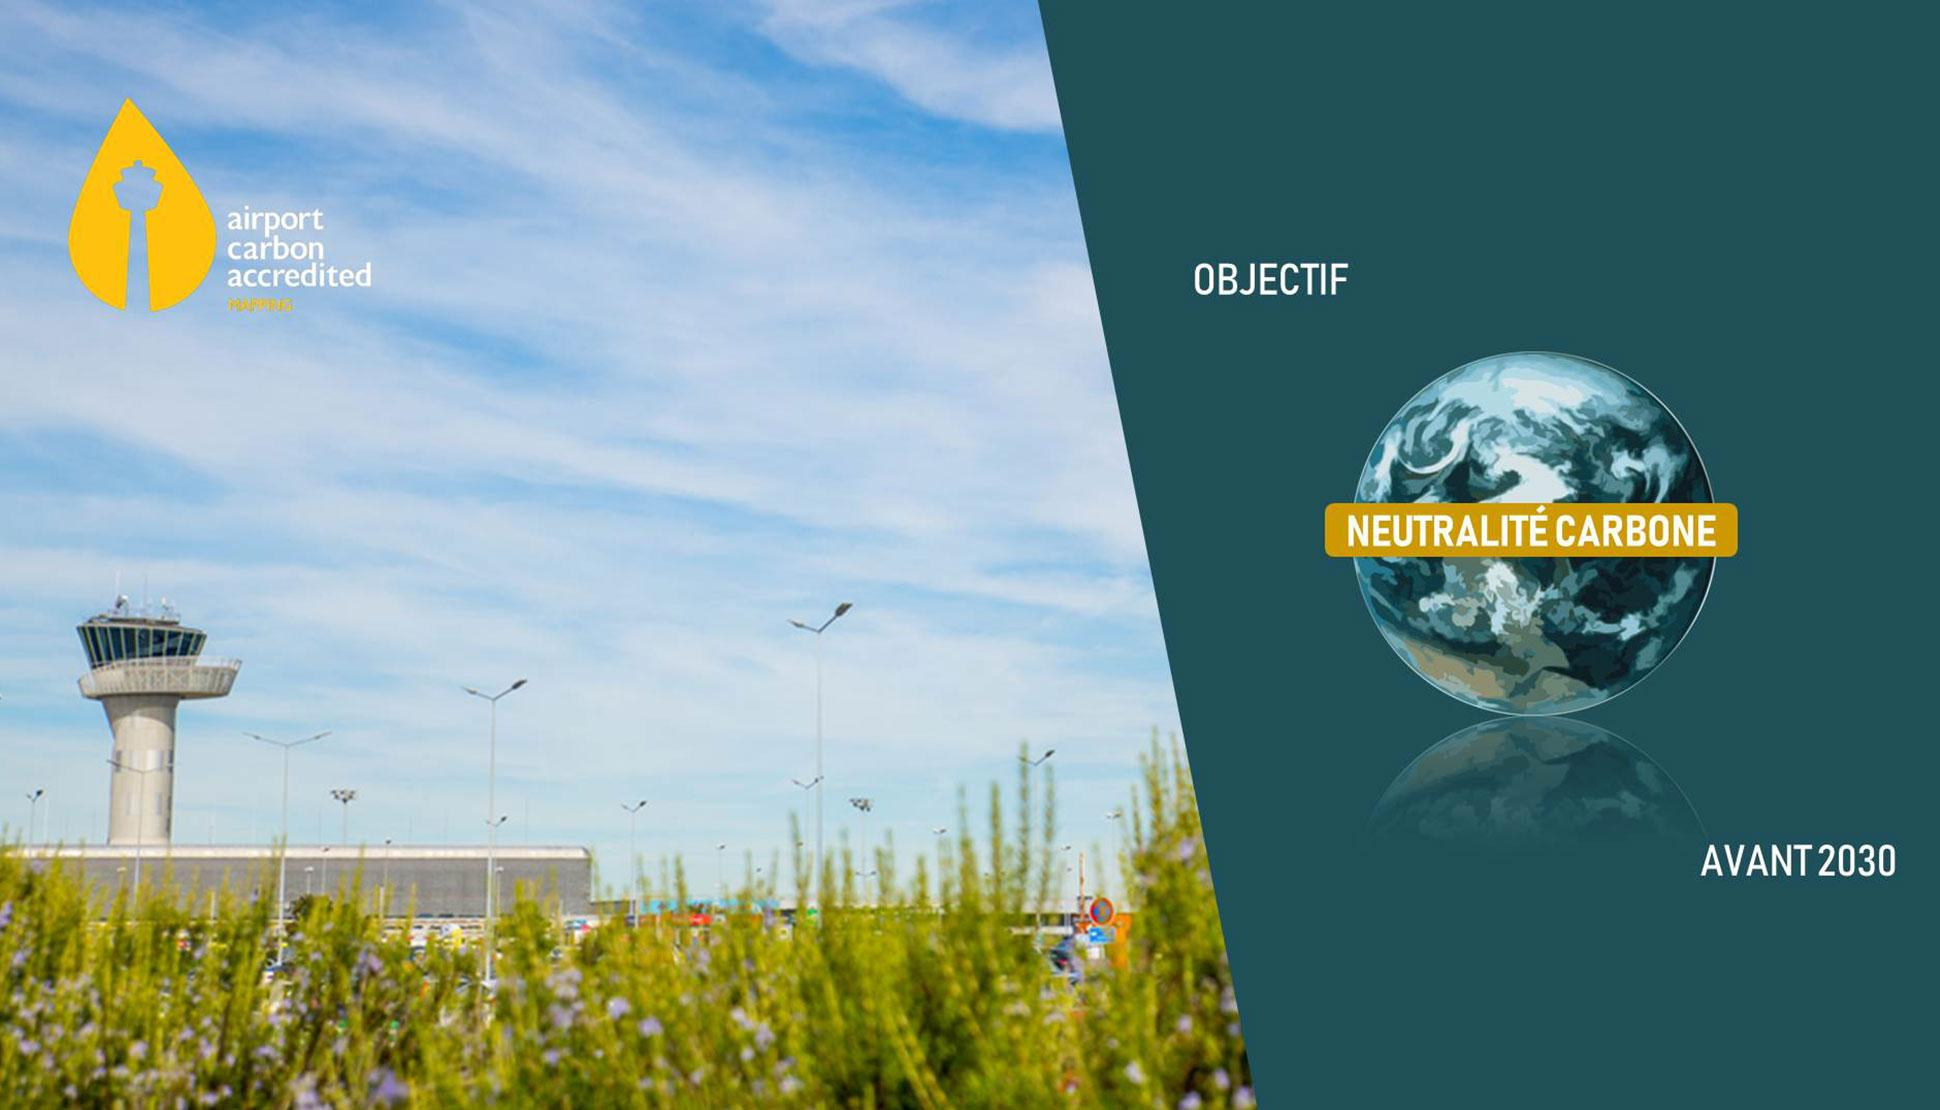
\includegraphics[width=12cm]{Images/aca2030.jpg}
  \caption{Airport Carbon Accreditation}
  \label{fig:aca2030}
\end{figure}


L'aéroport ne se limite pas à ce seul programme. Il a décidé d'agir de manière importante sur son activité afin de réduire leur pollution.


Concernant le côté ville, des actions comme le tri sélectif sont effectuées dans tout l'aéroport : pour le public mais également pour les salariés. SA ADBM rembourse 80\% du prix de l'abonnement de transports en communs aux salariés si celui-ci sert à venir travailler, afin de lutter contre la pollution automobile.


SA ADBM possède de nombreux véhicules : bus (navettes entre les parkings et l'aérogare), voitures de services, voitures d'astreintes. Tout ces véhicules polluent et le service environnement de l'aéroport le sait . Une nouvelle règle a été instaurée : lors d'un achat/remplacement de véhicule, celui-ci doit être électrique ou hybride (selon les besoins). Cela permettra de réduire la consommation liée aux transports.\newline


Dans un objectif de réduction des émissions de carbone côté piste, la mise en place d’équipements d’alimentation électriques en « 400 Hertz » a été effectuée en remplacement des groupes électrogènes à moteur thermique. Ils servent notamment à garder du courant dans l'appareil lorsqu'il est stationné.


De plus, tout nouveau bâtiment (comme le Satellite 3), doit être construit avec la norme Haute Qualité Environnementale et selon des critères renforcés de qualité de service. Cela permettra de réduire la consommation d'énergie sur le long terme.\newline


L'entreprise travaille également à la pose de panneaux photovoltaïques un peu partout sur la plateforme aéroportuaire : façades des Halls A et B, accès aux Parkings et alentours des pistes.


La plateforme aéroportuaire fait également attention à ses consommations d'eau. Des "Urinoirs Secs" ont été installés en 2019, et après 1 an ils ont permis d'économiser 1 million de litres d'eau. Leur installation continue donc progressivement.
De plus, la SA ADBM a un système de récupération d'eau de pluie et de récupération des eaux servant à l'entraînement des pompiers de la plateforme.\newline


La végétalisation est un projet qui tient à coeur aux responsables environnement. Lors de l'arrivée du Tramway en 2022, les abords seront végétalisés avec l'exigence « zéro phytosanitaire ».\newline


La faune et la flore sont des points très importants lors de l'évolution des infrastructures. Avant de lancer une construction, la SA ADBM fait intervenir un prestataire afin de réaliser une étude du terrain et étudier les conséquences sur l'environnement.
Concernant le projet "45ème Parallèle", c'est la société Thallium qui s'en est chargé. Ils étudient la faune et la flore locale et éditent un rapport sur ce qui doit être fait avant la construction.

Voici une carte réalisée pour ce projet :

\begin{figure}[hbt!]
  \centering
  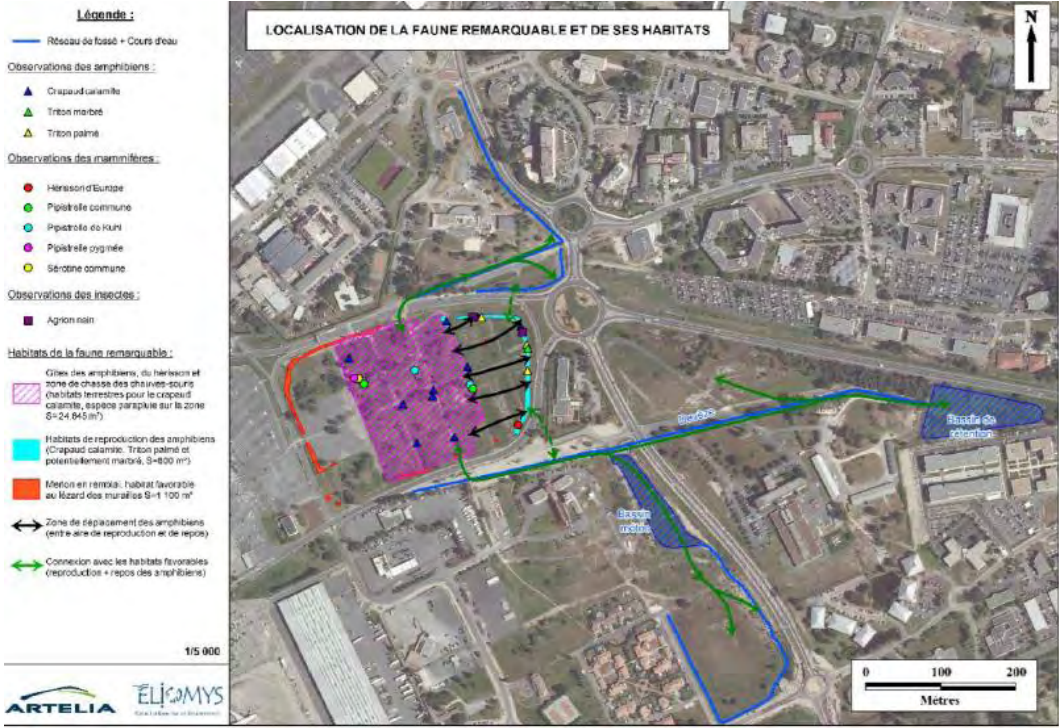
\includegraphics[width=14cm]{Images/carteenvironnement.png}
  \caption{Carte de localisation de la faune et de la flore}
  \label{fig:crapeau}
\end{figure}

Concernant la faune, SA ADBM a également installé des ruches dans un endroit végétalisé éloigné de la vue du public. Une population de 150 000 abeilles s'y est installée, puis des ruches additionnelles ont été ajoutées. Il y a désormais 300 000 spécimens. Des apiculteurs viennent régulièrement s'occuper des ruches et d'ici quelques mois plusieurs kilogrammes de miel de l'Aéroport de Bordeaux-Mérignac seront produits.

 \begin{figure}[hbt!]
   \centering
   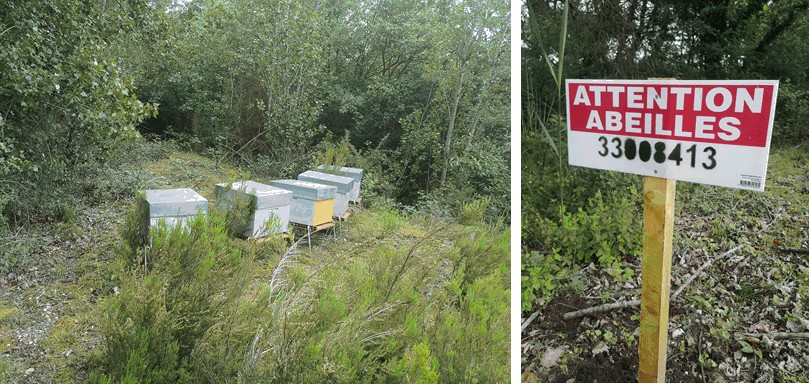
\includegraphics[width=14cm]{Images/ruches.jpg}
   \caption{Ruches}
   \label{fig:abeilles}
 \end{figure}

